
%                      Template Naskah Skripsi
%               	Berdasarkan format JTETI FT UGM
% 						(c) @gunturdputra 2014
%-------------------------------------------------------------------------------

%Template pembuatan naskah skripsi.
\documentclass{jtetiskripsi}

%Untuk prefiks pada daftar gambar dan tabel
\usepackage[titles]{tocloft}
\renewcommand\cftfigpresnum{Gambar\  }
\renewcommand\cfttabpresnum{Tabel\   }

%Untuk hyperlink dan table of content
\usepackage[hidelinks]{hyperref}
\newlength{\mylenf}
\settowidth{\mylenf}{\cftfigpresnum}
\setlength{\cftfignumwidth}{\dimexpr\mylenf+2em}
\setlength{\cfttabnumwidth}{\dimexpr\mylenf+2em}

%Untuk Bold Face dan centering pada Keterangan
\usepackage[labelfont=bf,justification=centering]{caption}

%Untuk caption dan subcaption
\usepackage{caption}
\usepackage{subcaption}

%pdf
\usepackage{pdfpages}

%table
\usepackage{array}
\usepackage{longtable}
\newcolumntype{P}[1]{>{\centering\arraybackslash}p{#1}}
\usepackage{graphics}
\usepackage{wrapfig}

%bibliography
\usepackage[
  style=authoryear-icomp,
  maxcitenames=1,
  isbn=false,
  doi=false,
  url=false,
  autolang=other,
  hyperref=true,
  sortcites=true,
  bibwarn=true,
  firstinits=true,
  autolang=other,
]{biblatex}
\DefineBibliographyStrings{english}{%
  andothers = {et al\adddot,\addspace},
}
\DeclareFieldFormat{citehyperref}{%
  \DeclareFieldAlias{bibhyperref}{noformat}% Avoid nested links
  \bibhyperref{#1}}

\DeclareFieldFormat{textcitehyperref}{%
  \DeclareFieldAlias{bibhyperref}{noformat}% Avoid nested links
  \bibhyperref{%
    #1%
    \ifbool{cbx:parens}
      {\bibcloseparen\global\boolfalse{cbx:parens}}
      {}}}

\savebibmacro{cite}
\savebibmacro{textcite}

\renewbibmacro*{cite}{%
  \printtext[citehyperref]{%
    \restorebibmacro{cite}%
    \usebibmacro{cite}}}

\renewbibmacro*{textcite}{%
  \ifboolexpr{
    ( not test {\iffieldundef{prenote}} and
      test {\ifnumequal{\value{citecount}}{1}} )
    or
    ( not test {\iffieldundef{postnote}} and
      test {\ifnumequal{\value{citecount}}{\value{citetotal}}} )
  }
    {\DeclareFieldAlias{textcitehyperref}{noformat}}
    {}%
  \printtext[textcitehyperref]{%
    \restorebibmacro{textcite}%
    \usebibmacro{textcite}}}
\addbibresource{daftar-pustaka.bib}

%equation
\usepackage{amsmath}

%algorithm & syntax
\usepackage{algorithm}
\usepackage{algpseudocode}
\algnewcommand\algorithmicforeach{\textbf{for each:}}
\algnewcommand\ForEach{\item[ \algorithmicforeach]}
\algdef{SE}[DOWHILE]{Do}{doWhile}{\algorithmicdo}[1]{\algorithmicwhile\ #1}%
\newenvironment{conditions}
  {\par\vspace{\abovedisplayskip}\noindent\begin{tabular}{>{$}l<{$} @{${}={}$} l}}
  {\end{tabular}\par\vspace{\belowdisplayskip}}

%code
\usepackage{listings}
\usepackage{xcolor}
\definecolor{codegreen}{rgb}{0,0.6,0}
\definecolor{codegray}{rgb}{0.5,0.5,0.5}
\definecolor{codepurple}{rgb}{0.58,0,0.82}
\lstdefinestyle{mystyle}{
    commentstyle=\color{codegreen},
    keywordstyle=\color{magenta},
    numberstyle=\tiny\color{codegray},
    stringstyle=\color{codepurple},
    basicstyle=\ttfamily\footnotesize,
    frame=single,
    breakatwhitespace=false,
    breaklines=true,
    captionpos=b,
    keepspaces=true,
    numbersep=5pt,
    showspaces=false,
    showstringspaces=false,
    showtabs=false,
    tabsize=2
}
\lstset{style=mystyle}
\makeatletter
\def\thechapter{\@Roman\c@chapter}
\AtBeginDocument{%
  \def\thelstlisting{\@arabic\c@chapter.\@arabic\c@lstlisting}}
\makeatother

%Create a new minipage environment where paragraphs have indents
\newlength{\currentparindent}
\newenvironment{minipageparindent}[2][c]
  {\setlength{\currentparindent}{\parindent}% save the value
   \noindent\begin{minipage}[#1]{#2}% open the minipage
   \setlength{\parindent}{\currentparindent}% restore the value
  }
  {\end{minipage}}

%Create an environment that creates a paragraph with a picture next to it, both being aligned at the top.
\newenvironment{pictureparagraph}[1]    %argument is an 'includegraphics' command
    {\newcommand\picturetoplace{#1}     % using variable directly gives an error
    \begin{minipageparindent}[t]{0.7\textwidth} %
    \vspace{0pt}    %Make sure that the top base is at the absolute top
    }   
    {
    \end{minipageparindent}
    \begin{minipage}[t]{0.3\textwidth}
    \vspace{0pt}    %Make sure that the top base is at the absolute top of the minipage
    \picturetoplace
    \end{minipage}\\}


%-----------------------------------------------------------------
%Disini awal masukan untuk data proposal skripsi
%-----------------------------------------------------------------
\titleind{Implementasi Modul Indexing Pada Search Engine Telusuri Dengan 
Integrasi Inverted Index dan Generalized Suffix Tree Untuk Mereduksi Waktu 
Pencarian}

\fullname{Mochammad Hanif Ramadhan}

\idnum{1313619025}

\approvaldate{21 Agustus 2023}

\degree{Sarjana Ilmu Komputer}

\yearsubmit{2023}

\program{Ilmu Komputer}

\dept{Ilmu Komputer}

\firstsupervisor{Muhammad Eka Suryana, M. Kom.}
\firstnip{198512232012121002}

\secondsupervisor{Med Irzal, M. Kom.}
\secondnip{197706152003121001}

%-----------------------------------------------------------------
%Disini akhir masukan untuk data proposal skripsi
%-----------------------------------------------------------------

\tolerance=1
\emergencystretch=\maxdimen{}
\hyphenpenalty=10000
\hbadness=10000

\begin{document}

\cover{}
\clearpage{}
\setcounter{page}{1}
%-----------------------------------------------------------------

%-----------------------------------------------------------------
%Disini akhir masukan untuk muka skripsi
%-----------------------------------------------------------------
% % \chapter*{\centering{\large{LEMBAR PERSETUJUAN}}}
\chapter*{\centering{\large{LEMBAR PENGESAHAN}}}
\thispagestyle{empty} {\bf }Dengan ini saya mahasiswa Fakultas
Matematika dan Ilmu Pengetahuan Alam, Universitas Negeri Jakarta

\vskip3mm

\begin{tabular}{ll}
  Nama & : Mochammad Hanif Ramadhan \\
  No. Registrasi & : 1313619025 \\
  Program Studi & : Ilmu Komputer \\
  Judul & : Implementasi Modul Indexing Pada Search Engine \\ & \hspace{0.2cm}
  Telusuri Dengan Integrasi Inverted Index dan Generalized Suffix \\ & \hspace{0.2cm}
  Tree Untuk Mereduksi Waktu Pencarian
\end{tabular}

\vskip3mm

% \noindent \hskip10mm Menyatakan bahwa proposal ini telah siap diajukan untuk seminar pra skripsi.
\begin{center}
Menyatakan bahwa skripsi ini telah siap diajukan untuk sidang skripsi.
\end{center}



\begin{center}
\vskip3mm

Menyetujui,

\vskip3mm
\begin{spacing}{1.25}

\begin{tabular}{ccc}
  \hskip-2mm Dosen Pembimbing I & \qquad \qquad \qquad \qquad \qquad & \hskip-6mm Dosen Pembimbing II \\
   &  &  \\
   &  &  \\
   &  &  \\
   &  &  \\
  \hskip-2mm \underline{\textbf{Muhammad Eka Suryana, M.Kom}} &  & \hskip-6mm \underline{\textbf{Med
  Irzal, M.Kom}} \\
  \hskip-2mm NIP. 19770615 200312 1 001 &  & \hskip-6mm NIP. 19851223 201212 
  1 002	 \\
\end{tabular}
\end{spacing}
\end{center}
\vskip3mm
\begin{center}
Mengetahui, \\
Koordinator Program Studi Ilmu Komputer
\end{center}
\begin{spacing}{1.25}
{ \ }
\\
\\
{ \ }\begin{center}
\underline{\textbf{Dr. Ria Arafiyah, M.Si}} \\
{NIP. 19751121 200501 2 004}
\end{center}
\end{spacing} 

% 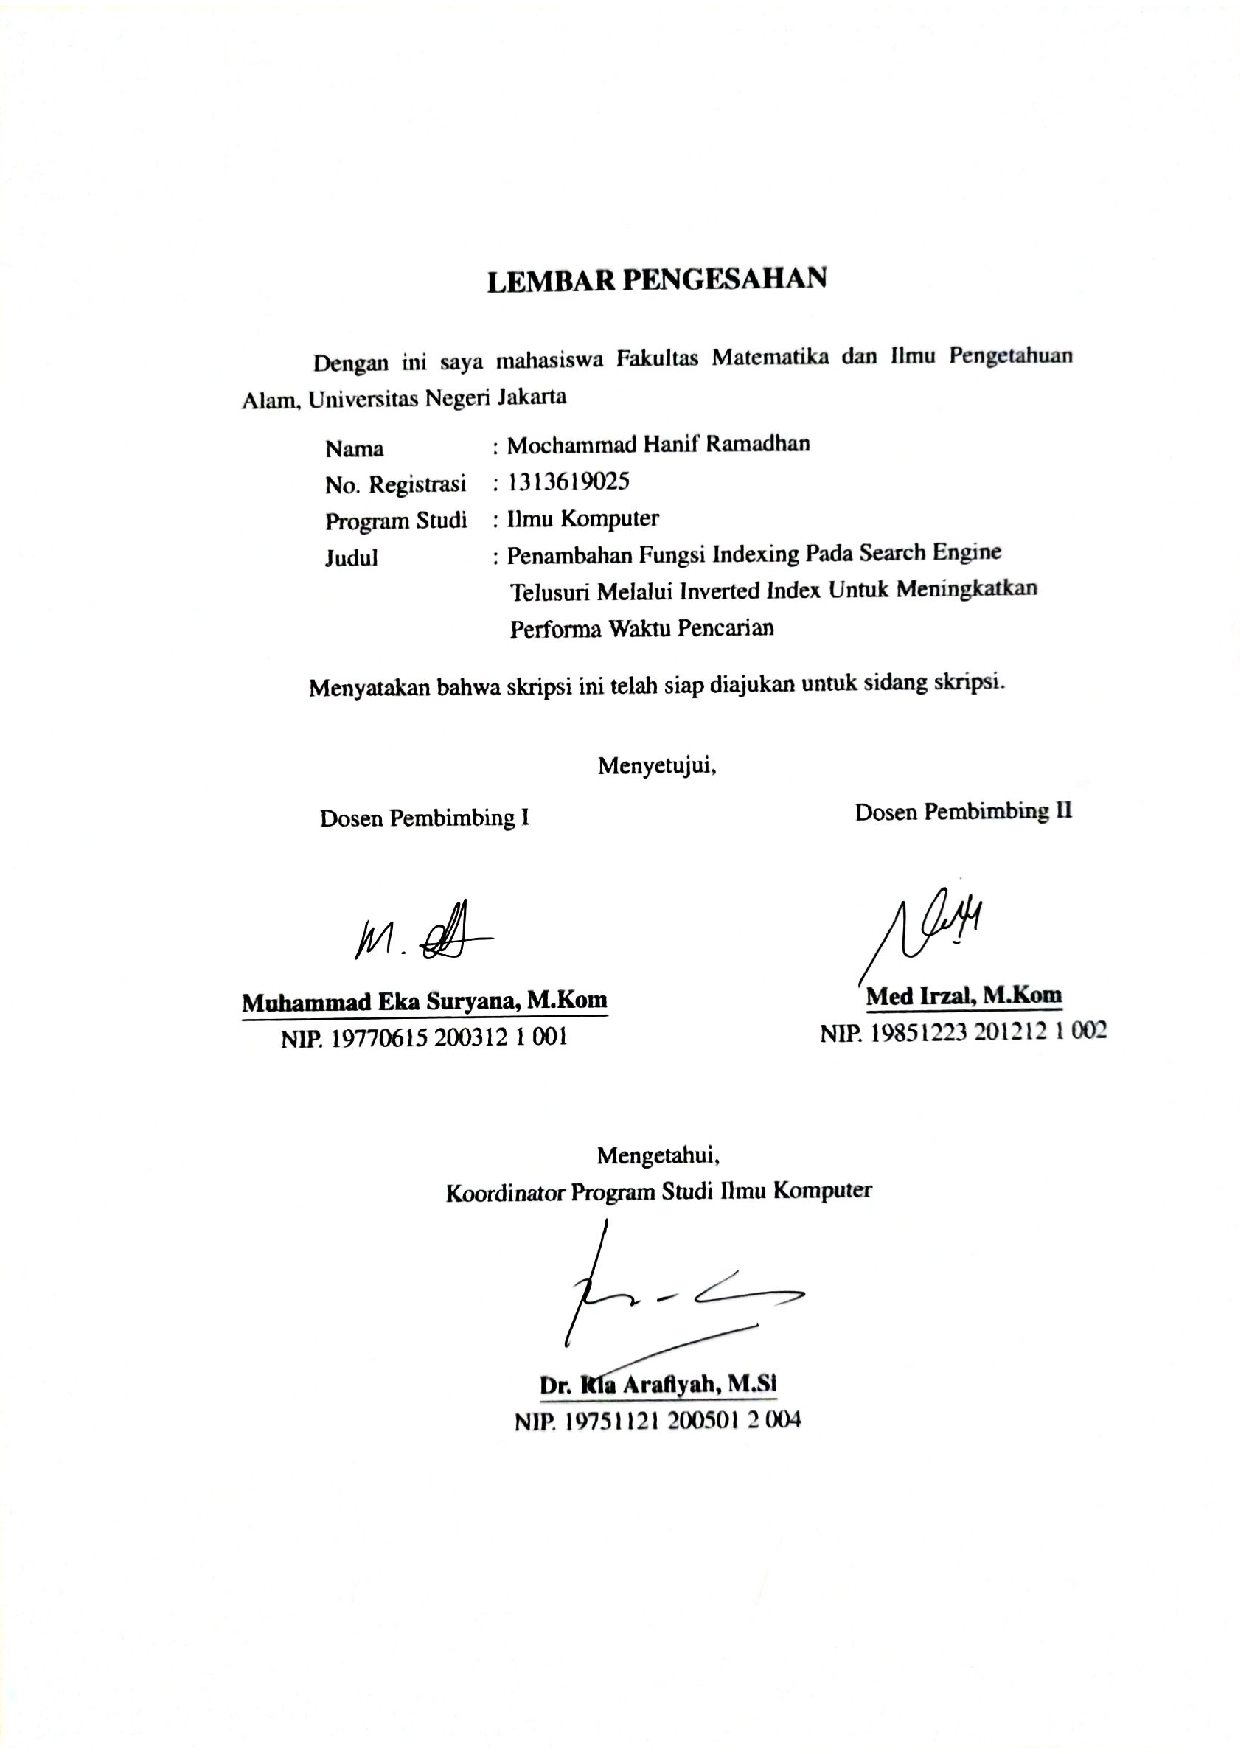
\includepdf[pages=-]{LembarPengesahan.pdf}
\chapter*{\centering{\large{LEMBAR PERNYATAAN}}}
\onehalfspacing{}

Saya menyatkan dengan sesungguhnya bahwa skripsi dengan judul
\textbf{"Implementasi Modul Indexing Pada Search Engine Telusuri Dengan
Integrasi Inverted Index Dan Generalized Suffix Tree Untuk Mereduksi Waktu
Pencarian"} yang disusun sebagai syarat untuk memperoleh gelar Sarjana Komputer
dari Program Studi Ilmu Komputer Universitas Negeri Jakarta adalah karya ilmiah
saya dengan arahan dari dosen pembimbing.

Sumber informasi yang diperoleh dari peneliti lain yang telah dipublikasikan 
yang disebutkan dalam teks Skripsi ini, telah dicantumkan dalam Daftar Pustaka 
sesuai dengan norma, kaidan dan etika penulisan ilmiah.

Jika dikemudian hari ditemukan sebagian besar skripsi ini bukan hasil karya saya 
sendiri dalam bagian-bagian tertentu, saya bersedia menerima sanksi pencabutan 
gelar akademik yang saya sanding dan sanksi-sanksi lainnya sesuai dengan 
peraturan perundang-undangan yang berlaku.

\vspace{4cm}

\begin{tabular}{p{7.5cm}c}
	&Jakarta, 21 Agustus 2023\\
	&\\
	&\\
	&\\
	&Mochammad Hanif Ramadhan
\end{tabular}


\chapter*{\centering{\large{KATA PENGANTAR}}}
\onehalfspacing{}
Puji syukur penulis panjatkan ke hadirat Allah SWT, karena dengan rahmat dan
karunia-Nya, penulis dapat menyelesaikan proposal skripsi yang berjudul
\textit{Implementasi Modul Indexing Pada Search Engine Telusuri Dengan Integrasi 
Inverted Index Dan Generalized Suffix Tree Untuk Mereduksi Waktu Pencarian}.

Keberhasilan dalam penyusunan proposal skripsi ini tidak lepas dari bantuan
berbagai pihak yang mana dengan tulus dan ikhlas memberikan masukan guna
sempurnanya proposal skripsi ini. Oleh karena itu dalam kesempatan ini, dengan
kerendahan hati penulis mengucapkan banyak terima kasih kepada:

\begin{enumerate}

	\item{Yth. Para petinggi di lingkungan FMIPA Universitas Negeri Jakarta.}
	\item{Yth. Ibu Dr. Ria Arafiyah, M.Si selaku Koordinator Program Studi Ilmu
		Komputer.}
	\item{Yth. Bapak Muhammad Eka Suryana, M.Kom selaku Dosen Pembimbing I yang
		telah membimbing, mengarahkan, serta memberikan saran dan koreksi terhadap
		proposal skripsi ini.}
	\item{Yth. Bapak Med Irzal, M.Kom selaku Dosen Pembimbing II yang telah
		membimbing, mengarahkan, serta memberikan saran dan koreksi terhadap
		proposal skripsi ini.}
	\item{Kedua orang tua dan kakak penulis yang telah mendukung dan memberikan 
		semangat serta doa untuk penulis.}
	\item{Wulan sebagai seseorang yang mau mendengarkan keluh kesah dan mendukung 
		penulis.}
	\item{Teman-teman Warung Tegang yang walau dengan segala keanehannya selalu
		memberikan semangat dan motivasi bagi penulis}
	\item{Teman-teman SMAN 68 yang seringkali menemani penulis bertukar pikiran 
		ketika beristirahat sejenak selama penulisan}
	\item{Teman-teman Program Studi Ilmu Komputer 2019 yang telah memberikan 
		dukungan dan memiliki andil dalam penulisan proposal skripsi ini.}
	\item{Kedua kucing milik Pak Eka yang seringkali menghibur penulis selama 
		melaksanakan bimbingan di Jasinga}
	
\end{enumerate}

Penulis menyadari bahwa penyusunan proposal skripsi ini masih jauh dari sempurna
karena keterbatasan ilmu dan pengalaman yang dimiliki. Oleh karenanya, kritik
dan saran yang bersifat membangun akan penulis terima dengan senang hati. Akhir
kata, penulis berharap tugas akhir ini bisa bermanfaat bagi semua pihak
khususnya penulis sendiri. Semoga Allah SWT senantiasa membalas kebaikan semua
pihak yang telah membantu penulis dalam menyelesaikan proposal skripsi ini.

\vspace{4cm}

\begin{tabular}{p{7.5cm}c}
	&Jakarta, 21 Agustus 2023\\
	&\\
	&\\
	&\\
	&Mochammad Hanif Ramadhan
\end{tabular}

\addcontentsline{toc}{chapter}{KATA PENGANTAR}
\chapter*{\textbf{ABSTRAK}}

\textbf{MOCHAMMAD HANIF RAMADHAN}. Implementasi Modul Indexing Pada Search 
Engine Telusuri Dengan Integrasi Inverted Index Dan Generalized Suffix Tree 
Untuk Mereduksi Waktu Pencarian. Skripsi. Program Studi Ilmu Komputer. Fakultas
Matematika dan Ilmu Pengetahuan Alam, Universitas Negeri Jakarta. Agustus 2023.
Di bawah bimbingan Muhammad Eka Suryana, M.Kom dan Med Irzal, M.Kom.

\vspace{5mm}
\noindent{}
Mesin pencari atau \emph{search engine} adalah program komputer yang digunakan 
untuk melakukan pencarian situs web. Pencarian dapat dilakukan dengan 
mengumpulkan informasi tentang halaman web terlebih dahulu. Karena ukuran data 
yang besar sebagai sumber informasi utama bagi mesin pencari, penggunaan
\textit{index} bisa dimanfaatkan untuk mereduksi waktu pencarian.  Penelitian
ini merupakan bagian dari rangkaian penelitian mesin pencari \textit{Telusuri},
dan bertujuan untuk membuat implementasi \textit{index} berdasarkan struktur
\textit{inverted index}, yaitu struktur \textit{index} yang digunakan oleh mesin
pencari \textit{Google}, dan melakukan integrasi dengan struktur
\textit{Generalized Suffix Tree}. Tujuan utamanya adalah untuk mereduksi waktu
pencarian suatu \textit{keyword} dan memberikan peringkat terhadap dokumen
berdasarkan kesesuaian antara informasi dalam dokumen dengan teks yang
dimasukkan oleh pengguna. Hasil akhir dari implementasi modul menunjukkan
reduksi waktu yang signifikan, berkisar antara 89 - 98\%.

\vspace{5mm}
\noindent{}
\textbf{Kata kunci}: \textit{mesin pencari, indeks, basis data, teori informasi}

\addcontentsline{toc}{chapter}{ABSTRAK}
\chapter*{\textbf{ABSTRACT}}

\textbf{MOCHAMMAD HANIF RAMADHAN}. Implementasi Modul Indexing Pada Search 
Engine Telusuri Dengan Integrasi Inverted Index Dan Generalized Suffix Tree 
Untuk Mereduksi Waktu Pencarian. Mini Thesis. Computer Science. Faculty of 
Mathematics and Natural Sciences, Universitas Negeri Jakarta. August 2023.
Under guidance from Muhammad Eka Suryana, M.Kom and Med Irzal, M.Kom.

\vspace{5mm}
\noindent{}
Search engine is a computer program that is used to search for a webpage. Before 
searching can be done, it is required to gather informatoin about the webpage 
first. Due to the large collection of data needed for a search engine to be 
usable, indexes can be used to reduce time to retrieve information. This 
research is a part of a longer research for \textit{Telusuri} search engine, and
aims to implement an index structure based on inverted index form, which are 
used by \textit{Google}, and integrates it with the \textit{Generalized Suffix 
Tree}. The goals is to reduce the time taken to get informations from a given 
keyword and ranks the result based on the relevancy between the webpage and the 
input keyword. The index implementations are shown to be able to reduce the time 
taken significantly, ranging from 89 to 98\%.

\vspace{5mm}
\noindent{}
\textbf{Kata kunci}: \textit{search engine, indexing, database, information 
retrieval, tree}

\addcontentsline{toc}{chapter}{ABSTRACT}
\singlespacing{}
\tableofcontents{}
\addcontentsline{toc}{chapter}{DAFTAR ISI}
\listoffigures{}
\addcontentsline{toc}{chapter}{DAFTAR GAMBAR}
\listoftables{}
\addcontentsline{toc}{chapter}{DAFTAR TABEL}

\begin{counterpage}
\end{counterpage}
%Disini awal masukan untuk Bab
%-----------------------------------------------------------------
\onehalfspacing{}
%!TEX root = ./template-skripsi.tex
%-------------------------------------------------------------------------------
% 								BAB I
% 							LATAR BELAKANG
%-------------------------------------------------------------------------------

\chapter{PENDAHULUAN}

\section{Latar Belakang Masalah}

% Intro
Mesin pencari atau \emph{search engine} adalah program komputer yang digunakan 
untuk melakukan pencarian situs web. Pada awal kemunculannya, mesin pencari
lebih diperuntukkan bagi kalangan akademisi untuk mencari jurnal atau dokumen
akademik lainnya. Namun, seiring dengan meluasnya adopsi internet ke berbagai
lapisan masyarakat, mesin pencari memiliki peran yang lebih besar dalam
penggunaan internet. Mesin pencari menjadi sarana utama dalam pencarian
informasi.

% Sejarah mesin pencari
Bila dilihat dari penggunaannya, mesin pencari bekerja dengan cara mengolah
\emph{query} yang diberikan oleh pengguna dan menampilkan hasil terkait
informasi tertentu di internet yang paling sesuai dengan \emph{query} tersebut.
Tetapi mesin pencari tidak dapat langsung mencari ke seluruh halaman yang ada
pada internet. Mesin pencari membutuhkan database yang berisi informasi pada
halaman yang tersebar di seluruh jaringan internet. 

Ketika internet masih memiliki lingkup pengguna yang kecil, metode pengumpulan
data untuk database mesin pencari masih bersifat manual. \emph{Archie}, mesin
pencari pertama, mengumpulkan data dengan cara mencari daftar situs yang
tersedia secara publik menggunakan protokol \emph{Telnet} dan memperbarui-nya
secara berkala. \emph{Yahoo} pada awal kemunculannya mempekerjakan beberapa
kurator untuk mereview situs mana yang berkualitas untuk kemudian ditambahkan
secara manual kedalam database.  Semakin tingginya adopsi internet membuat
jumlah data pada internet meledak. Hal ini berakibat pada diperlukannya metode
pengumpulan data yang lebih efisien dan metode penerimaan informasi yang lebih
cepat.

% Arsitektur Google
Mesin pencari membutuhkan serangkaian proses yang perlu dilakukan sebelum dapat
menerima \emph{query} terkait informasi tertentu. Pada arsitektur \emph{Google},
terdapat beberapa komponen yang memiliki tugasnya tersendiri. Pertama,
diperlukan proses \emph{crawling} untuk mendapatkan kumpulan \emph{web page}.
Proses ini dilakukan oleh beberapa \emph{crawler}.

% Google menggunakan algoritma indexing sendiri.
\emph{Google}, mesin pencari paling populer saat ini, mengungkapkan detail dari
arsitektur yang digunakan dalam sebuah paper yang di rilis pada tahun 1998.
Arsitektur \emph{Google} terdiri dari beberapa komponen utama seperti
\emph{crawler}, modul \emph{indexer}, modul pemeringkatan \emph{PageRank} dan
modul pencari.

Implementasi ulang arsitektur \emph{Google} secara menyeluruh cukup sulit
dilakukan banyak detail dari arsitektur yang tidak tercantum dalam paper nya.
Selain itu \emph{Google} juga banyak menggunakan teknologi yang telah
dioptimalkan untuk kebutuhan mesin pencari baik dari segi performa maupun
penggunaan media penyimpanannya, tetapi kode programnya tidak dapat diakses.

% Arsitektur Lazuardy
Upaya implementasi ulang arsitektur \emph{Google} telah dilakukan oleh Lazuardy
Khatulistiwa dalam penelitiannya yang berjudul \emph{Perancangan Arsitektur
Search Engine Dengan Mengintegrasikan Web Crawler, Algoritma Page Ranking, dan
Document Ranking}. Arsitektur tersebut merupakan pengembangan dari penelitian
yang dilakukan oleh Muhammad Fathan yang menghasilkan \emph{web crawler}.
\emph{Web crawler} bertugas mengumpulkan halaman web berdasarkan
\emph{entrypoint} tertentu.  Halaman web tersebut kemudian di ekstrak dan
dikumpulkan daftar kata yang termuat pada halaman web tersebut serta
\emph{outgoing link} yang merujuk kepada halaman web lain. Kedua data tersebut
kemudian disimpan pada database \emph{MySQL}.

Data yang tersimpan pada database selanjutnya di proses oleh modul
\emph{PageRank}. Modul \emph{PageRank} menghitung peringkat suatu halaman web
berdasarkan seberapa banyak halaman web lain yang merujuk kepada halaman web
tersebut. Setelah kalkulasi peringkat halaman, data akan diolah oleh modul
\emph{TF-IDF}. Modul \emph{TF-IDF} akan menghitung bobot kata pada dokumen
berdasarkan frekuensi kemunculan kata tersebut dalam suatu dokumen tertentu dan
jumlah dokumen yang mengandung kata tersebut. Hasil perhitungan skor dari modul
\emph{PageRank} dan \emph{TF-IDF} kemudian akan digabungkan dengan menggunakan
algoritma \emph{similarity scoring} yang akan menghasilkan skor relevansi suatu
halaman.

% Kekurangan dari arsitektur existing terutama pada bagian indexing
Hasil riset yang telah dilakukan oleh Lazuardy masih memiliki kekurangan, dan
implementasinya juga cukup berbeda dibandingkan dengan arsitektur milik
\emph{Google} karena keterbatasan detailnya.  Salah satu proses yang belum
dilakukan implementasi ulang adalah proses \emph{indexing}. \emph{Indexing}
adalah suatu proses pemetaan \emph{record} pada database dengan tujuan
mempercepat proses pengambilan \emph{record} dari database. Proses
\emph{indexing} akan menghasilkan \emph{index}, yaitu representasi data yang
merujuk pada lokasi data yang lebih lengkap pada database. Konsep \emph{index}
disini hampir sama dengan index yang biasa ditemukan di bagian belakang buku.

% Penjelasan terkait indexing
Representasi data oleh \emph{index} memiliki tingkat akurasi lokasi data
(\emph{granularity}) yang dapat diatur, seperti suatu frase dalam suatu
paragraf, atau unit data yang lebih kecil seperti satu kata tertentu saja.
Pemilihan tingkat \emph{granularity} dapat mempengaruhi performa dan akurasi
dari proses pengambilan data. Sebagai contoh, penggunaan \emph{synonym ring}
yang dapat melakukan pengelompokan kata yang bermakna sama seperti
\emph{WordNet} dapat memberikan hasil yang lebih baik dibandingkan dengan hanya
menggunakan potongan kata biasa~\cite{gonzalo1998wordnet}.

% Indexing untuk penyimpanan teks
Terdapat berbagai implementasi \emph{index} yang disesuaikan dengan jenis data
yang disimpan pada database. Mesin pencari membutuhkan implementasi \emph{index}
yang dioptimalkan untuk teks secara menyeluruh. Dalam artikel yang berjudul
\emph{An Efficient Indexing Technique for Full-Text Database Systems}, 
implementasi \emph{index} yang difokuskan kepada penyimpanan teks setidaknya
perlu melakukan tiga hal secara efisien. Yang pertama adalah mendukung
pengambilan dokumen berdasarkan \emph{query} berupa beberapa kata yang
digabungkan oleh operator logika. Yang kedua adalah memiliki kemampuan untuk
menambahkan \emph{record} baru secara efisien. Yang ketiga adalah kemampuan
untuk membuat pemeringkatan terhadap \emph{record} yang ada apabila tidak ada
data yang memenuhi \emph{query} secara penuh~\cite{zobel1992efficient}.

% Prinsip kerja
Dari persyaratan diatas, solusi yang umum digunakan untuk database penyimpanan
teks adalah \emph{inverted file index}. Wujud dari \emph{inverted file index}
adalah daftar yang memuat kata dan posisinya dalam dokumen yang diurutkan
berdasarkan kata.  Untuk mendapatkan daftar kata pada dokumen, dibutuhkan
\emph{lexicon} yang memuat seluruh kata yang muncul pada database
~\cite{hersh2001gigabytes}.

Penelitian tentang struktur data untuk keperluan \emph{indexing} telah dilakukan
oleh Zaidan yang berjudul \emph{Perancangan Modul Pengindeks Pada Search Engine
Berupa Induced Generalized Suffix Tree Untuk Keperluan Perangkingan Dokumen}.
Penelitian tersebut menggunakan \emph{generalized suffix tree} (\emph{GST})
sebagai alternatif dari \emph{inverted index} yang sudah umum digunakan sebagai
stuktur data \emph{index}. \emph{GST} diklaim mampu memberikan performa yang
lebih baik.

% Pross indexing Google
Proses \emph{indexing} yang akan di replika akan menggunakan detail yang
terbatas yang dapat diakses pada \emph{paper Google}.  Untuk memroses
\emph{query}, \emph{Google} melakukan beberapa langkah berikut.  Pertama,
\emph{query} dipotong per kata. Setiap kata kemudian di konversi menjadi
\emph{wordID}, yang dapat mengidentifikasi suatu kata secara unik.

Dari kumpulan \emph{wordID} tersebut, untuk setiap kata akan dicari
kemunculannya pada permulaan daftar \emph{index} yang berisi judul dan
\emph{outgoing links}.  Pencarian dilakukan dengan proses \emph{scanning} secara
menyeluruh pada daftar \emph{index} sampai ditemukan dokumen yang memenuhi
seluruh kata pada \emph{query}. Untuk setiap dokumen yang ditemukan, akan
dihitung skor dokumen berdasarkan \emph{query} yang ada.

Jika telah sampai pada akhir daftar dokumen dan posisi pencarian berada pada
daftar judul dan \emph{outgoing links}, maka posisi akan berpindah ke daftar
kata pada seluruh dokumen, dan mulai melakukan pencarian dokumen lagi. Tetapi
jika belum mencapai akhir daftar dokumen, maka posisi pencarian akan diulang
dari posisi awal dan memulai pencarian lagi. Setelah seluruh daftar
\emph{index} dikunjungi, nantinya akan diakhiri dengan mengurutkan dokumen
berdasarkan skor.

Arsitektur yang dibuat saat ini menggunakan algoritma \emph{similarity scoring}
untuk mendapatkan nilai relevansi suatu halaman, dengan rumus:

\begin{equation}
	W = \alpha{} \cdot{} PR + \beta{} \cdot{} QR
\end{equation}

Dimana $W$ adalah skor relevansi suatu halaman, $\alpha{}$ adalah konstanta yang
bernilai $0.4$, $PR$ adalah nilai dari \emph{PageRank}, $\beta{}$ adalah
konstanta yang bernilai $0.6$ dan $QR$ adalah skor pemeringkatan \emph{query}
yang menggabungkan beberapa algoritma dengan rumus:

\begin{equation}
	QR = \beta{}_1 \cdot{} QR_1 + \cdots{} + \beta{}_N \cdot{} QR_N
\end{equation}

Dimana $QR_N$ dapat berupa hasil dari algoritma \emph{query ranking} yang
digunakan seperti \emph{TF-IDF} atau \emph{Skipgram}.

Implementasi dari proses \emph{indexing} nantinya dapat berperan sebagai
metode \emph{query ranking} yang berbeda, atau melakukan enkapsulasi nilai
\emph{query ranking} yang sudah ada.

\section{Rumusan Masalah}
Berdasarkan uraian pada latar belakang yang di utarakan di atas, maka perumusan
masalah pada penelitian ini adalah '\textbf{TODO}'

\section{Pembatasan Masalah}
Pembatasan masalah pada penelitian ini adalah pembuatan sebagian arsitektur
mesin pencari yaitu \emph{indexing}. Sistem \emph{indexing} yang akan dibuat
mengacu pada konsep arsitektur \emph{Google} awal.

\section{Tujuan Penelitian}
\begin{enumerate}
	\item Memahami arsitektur mesin pencari.
	\item Memahami cara kerja proses \emph{indexing}.
	\item Membuat implementasi \emph{indexing} untuk memenuhi kebutuhan mesin
		pencari.
\end{enumerate}

\section{Manfaat Penelitian}
\begin{enumerate}
	\item Bagi penulis (TODO)
		
	Menambah pengetahuan dibidang \emph{information retrieval} khususnya mengenai
		\emph{search engine} dan \emph{crawling}, mengasah kemampuan
		\emph{programming}, dan memperoleh gelar sarjana dibidang Ilmu Komputer.
		Selain itu, penulisan ini juga merupakan media bagi penulis untuk
		mengaplikasikan ilmu yang didapat di kampus ke kehidupan masyarakat.
		
	\item Bagi Universitas Negeri Jakarta (TODO)
	
	Menjadi pertimbangan dan evaluasi akademik khususnya Program Studi Ilmu
		Komputer dalam penyusunan skripsi sehingga dapat meningkatkan kualitas
		akademik di program studi Ilmu Komputer Universitas Negeri Jakarta serta
		meningkatkan kualitas lulusannya.
			
\end{enumerate}

% Baris ini digunakan untuk membantu dalam melakukan sitasi
% Karena diapit dengan comment, maka baris ini akan diabaikan
% oleh compiler LaTeX.
\begin{comment}
\bibliography{daftar-pustaka}
\end{comment}

 %!TEX root = ./template-skripsi.tex
%-------------------------------------------------------------------------------
%                            BAB II
%               KAJIAN TEORI
%-------------------------------------------------------------------------------

\chapter{KAJIAN PUSTAKA}

\section{Proses \emph{Indexing}}

\emph{Indexing} adalah proses pemetaan seluruh data pada \emph{database}.
Proses dimulai dengan mengambil data mentah dari \emph{repository}, yaitu tempat
penampungan data yang telah dikumpulkan oleh \emph{crawler}. Data tersebut
kemudian akan dipetakan sesuai dengan struktur index yang digunakan. Hasil dari
proses indexing adalah sebuah daftar \emph{index}, yang memiliki cara kerja yang
serupa dengan index yang biasa ditemui pada bagian belakang sebuah buku. Index
adalah suatu representasi data yang merujuk kepada lokasi data yang lebih
lengkap di dalam database.

Index merupakan komponen penting dalam suatu arsitektur mesin pencari.
Penggunaan index memberikan pengaruh signifikan dalam proses penerimaan data
dari database karena dapat mengurangi waktu akses \emph{storage}. Hal ini
sejalan dengan pola penggunaan mesin pencari, dimana mayoritas operasi yang
dilakukan adalah memberikan informasi berdasarkan \emph{query} dari pengguna.
Selain itu, representasi index tertentu juga dapat mempengaruhi pengolahan
\emph{query}, penggunaan ruang pada media penyimpanan dan akurasi dari hasil
\emph{query} tersebut.

% TODO Verif ke pak Eka apakah ini masih perlu atau tidak
% Terkait apakah database yang dibutuhkan adalah untuk full-text
Database yang digunakan oleh mesin pencari adalah database yang dirancang
untuk kebutuhan penyimpanan teks secara penuh. Untuk keperluan tersebut,
setidaknya terdapat tiga syarat yang perlu dipenuhi ketika ingin menentukan
representasi index.

\begin{enumerate}
  \item{Memungkinkan untuk mendapatkan data berdasarkan suatu query}

  Dari suatu query pencarian, database harus dapat memberikan hasil yang dapat
  memenuhi query tersebut. Pada konteks penerimaan data yang berbentuk teks,
  konjungsi query sangat umum digunakan. Dalam kasus ini, index harus mampu
  memberikan informasi apakah suatu \emph{record} mengandung kata tertentu, dan
  secara langsung mempengaruhi penentuan granularitas index.

  \item{Menambahkan \emph{record} baru secara efisien}

  Database yang hanya menyimpan teks umumnya digunakan untuk keperluan
  penyimpanan. Pada kasus mesin pencari, operasi yang sering dilakukan adalah
  penulisan data dari \emph{crawler} ke database dan pembacaan data berdasarkan
  query. Operasi untuk mengubah atau menghapus data jarang diperlukan, walaupun
  operasi tersebut tetap perlu didukung.

  \item{Memberikan skor terhadap hasil dari query yang bersifat `informal'}

  Pada kasus mesin pencari, pengguna seringkali memberikan query yang bersifat
  `informal', yaitu query yang tidak dapat dipenuhi seluruhnya oleh database.
  Dalam hal ini, database perlu memberikan hasil yang paling mendekati
  ekspektasi dari query tersebut dengan cara menyertakan nilai relevansi suatu
  data terhadap query.

  Mesin pencari setidaknya membutuhkan syarat pertama dan kedua untuk dipenuhi
  oleh database agar dapat digunakan di dunia nyata.

\end{enumerate}

\section{\emph{Repository}}

\emph{Repository} merupakan tempat penyimpanan seluruh kode HTML dari setiap
halaman web yang telah di-\emph{crawl}. Setiap dokumen memiliki data tambahan
yang disematkan kepadanya, yaitu nomor \emph{id} yang dibuatkan untuk dokumen
tersebut, panjang dari dokumen, dan \emph{URL} dari dokumen tersebut. Seluruh
data tersebut dikompres dengan library \emph{zlib} untuk mengurangi penggunaan
ruang pada \emph{repository}.

\section{Daftar URL}

Ketika mengolah data dari \emph{repository}, terdapat langkah tambahan yang
dilakukan jika menemui \emph{anchor text}. \emph{Anchor text} adalah teks berupa
URL yang merujuk kepada dokumen lain. Setiap \emph{anchor text} yang ditemukan
pada data dari \emph{repository} akan disimpan pada sebuah daftar URL\@. Daftar
ini nantinya 

\section{\emph{Document Index}}
\emph{Document index} menyimpan beberapa informasi tambahan pada setiap dokumen.
Setiap index akan memiliki nomor dokumen, status dokumen, alamat tempat dokumen
tersimpan di \emph{repository}, dan \emph{checksum}. Apabila pada suatu dokumen
telah dilakukan proses \emph{crawling}, maka akan disematkan data tambahan yang
berisi sepasang informasi berupa URL dan judul dari dokumen tersebut. Jika
belum melalui tahap \emph{crawling}, maka data tambahan tersebut hanya merujuk
kepada URL yang terdapat pada daftar URL\@.

\section{Daftar Kosakata}

Setiap hasil pengolahan data dari \emph{repository} akan memberikan daftar
kosakata yang bersifat unik. Daftar kosakata tersebut kemudian akan digabungkan
kedalam daftar kosakata yang menampung keseluruhan kosakata pada database yang
telah melalui proses \emph{indexing}.

Implementasi daftar kosakata ini terbagi menjadi dua bagian, yaitu daftar
kosakata itu sendiri dan daftar \emph{pointer} yang merujuk kepada dokumen
tempat kosakata itu berada. Selain itu, daftar kosakata dapat menyematkan
informasi tambahan seperti jumlah dokumen tempat kosakata tersebut muncul.

Untuk mencegah akses ke ruang penyimpanan yang berlebihan, salah satu syarat
dasar dari implementasi index adalah daftar seluruh kosakata dapat dimuat dalam
memori. Hal ini bertujuan untuk memastikan bahwa dalam situasi pencarian hasil
dengan query boolean, hanya membutuhkan setidaknya satu kali akses ke ruang
penyimpanan per kata.

\section{\emph{Inverted Index}}

\emph{Inverted index} merupakan jenis index yang memetakan potongan isi dari
suatu dokumen atau koleksi dokumen terhadap lokasi aslinya di dokumen atau
koleksi dokumen tersebut. Karena bentuk strukturnya, inverted index cocok
digunakan untuk kebutuhan penerimaan data berdasarkan query seperti mesin
pencari.

% \subsection{Struktur \emph{Inverted File Index}}

% Umumnya, implementasi dari inverted file index terdiri dari dua bagian, yaitu
% suatu struktur pencarian yang berisi seluruh kata pada seluruh dokumen yang
% telah di-\emph{index}, dan daftar dokumen yang telah di-\emph{index} beserta
% informasi lebih dalam terkait keberadaan kata pada struktur pencarian tersebut.

% Clarification
% jangan gunakan istilah struktur pencarian, pecah menjadi kegunaaannya
% masing-masing
% \subsubsection{Struktur Pencarian}
%
% Struktur pencarian terdiri dari dua bagian, yaitu daftar kata yang telah di
% index dan data tentang dokumen tempat kemunculan kata tersebut. Implementasi
% dari inverted file index mengasumsikan jika perangkat memiliki cukup memori
% untuk menampung seluruh struktur pencarian. Hal ini bertujuan untuk memastikan
% bahwa pencarian hasil yang dapat memenuhi suatu query boolean hanya membutuhkan
% setidaknya sekali akses ke ruang penyimpanan per kata.
%
% Akses terhadap ruang penyimpanan perlu dibatasi se minimal mungkin. Hal ini
% berdasarkan contoh kasus penggunaan database untuk kebutuhan mesin pencari.
% Karena jumlah data pada internet yang begitu banyak, proses pemetaan informasi
% dari seluruh internet akan menghasilkan data yang berukuran sangat besar. Hal
% ini akan menyebabkan proses baca ke ruang penyimpanan, walaupun hanya satu kali,
% memakan waktu yang tidak sebentar.

\subsection{Struktur Index}

Representasi dari kemunculan suatu kata pada dokumen, atau biasa disebut sebagai
\emph{hit}, memiliki beberapa data tertentu terkait kata yang dikandung. Setiap
\emph{hit} merepresentasikan suatu kemunculan kata beserta data berikut:

\begin{itemize}
  \item{Lokasi kata dalam dokumen}
  \item{Jenis \emph{font} yang digunakan}
  \item{Informasi terkait penggunaan huruf kapital}
\end{itemize}

\emph{Hit} terbagi menjadi tiga jenis berdasarkan lokasinya dalam struktur
halaman web. Yang pertama adalah \emph{fancy hit}, yaitu \emph{hit} yang berada
didalam \emph{URL}, judul halaman, atau \emph{meta tag}. Yang kedua adalah
\emph{anchor hit}, yaitu \emph{hit} yang khusus berada di dalam
\emph{anchor text} yang merupakan URL yang merujuk kepada dokumen atau halaman
lain. Yang ketiga adalah \emph{plain hit}, yaitu \emph{hit} yang berada diluar
lingkup dari \emph{fancy hit}.

Alokasi memori yang dibutuhkan untuk menyimpan sebuah \emph{hit} adalah 8 byte
atau 16 bit. Penggunaan bit tersebut berbeda tergantung dari jenis \emph{hit},
tetapi memiliki cara yang hampir sama dalam menggunakannya. 

Bit pertama digunakan sebagai penanda untuk penggunaan huruf kapital.
Selanjutnya, bit kedua hingga keempat digunakan sebagai penanda ukuran font yang
digunakan. Ukuran font ini bersifat relatif terhadap seluruh kata dalam dokumen.
Selain itu, nilai bit \emph{111} tidak digunakan sebagai ukuran penanda ukuran
font, namun digunakan sebagai penanda untuk \emph{fancy hit}. Bit kelima hingga
terakhir digunakan sebagai penanda posisi kata dalam dokumen. Karena
keterbatasan bit, posisi yang memiliki nilai lebih dari 4095 akan dianggap
bernilai 4096.

\begin{figure}[H]
  \centering{}
	\includegraphics[width=0.85\textwidth]{gambar/plain\-bit}
  \caption{Penggunaan alokasi memori dari \emph{plain hit}}
\end{figure}

Pada penggunaan \emph{fancy hit}, alokasi bit untuk penanda posisi dibagi
menjadi dua. Bit ke-9 hingga ke-12 digunakan sebagai penanda jenis dari
\emph{fancy hit}, sementara bit ke-13 hingga terakhir tetap digunakan sebagai
penanda posisi.

\begin{figure}[H]
  \centering{}
	\includegraphics[width=0.85\textwidth]{gambar/fancy\-bit}
  \caption{Penggunaan alokasi memori dari \emph{fancy hit}}
\end{figure}

Dari penggunaan \emph{fancy hit}, penggunaan \emph{anchor hit} membagi sisa
delapan bit terakhir menjadi dua, yaitu empat bit awal sebagai penanda posisi
dan empat bit terakhir sebagai nilai \emph{hash} dari dokumen dimana kata
tersebut berada.

\emph{Hit} dirangkai dengan menggunakan struktur \emph{linked list} agar
penambahan hit lebih mudah dilakukan ketika proses indexing ulang. Urutan dari
\emph{hit} dimulai dari kemunculan pertama kata tersebut dalam dokumen tertentu.
\emph{Hit} pertama dalam dokumen kemudian disambungkan ke \emph{id} dari dokumen
di depannya dengan menggunakan pointer.

\begin{figure}[H]
  \centering{}
	
\includegraphics[width=0.85\textwidth]{gambar/linkedListHit}
  \caption{Rangkaian \emph{hit} dengan struktur data \emph{linked list}}
\end{figure}

Iterasi terhadap seluruh \emph{hit} dapat dihindari dengan menyimpan total
\emph{hit} untuk suatu kata dalam suatu dokumen di depan rangkaian \emph{hit}.
Hal ini akan membuat proses penambahan \emph{hit} menjadi lebih efisien dan
memudahkan kalkulasi tingkat kepentingan suatu kata.

\begin{figure}[H]
  \centering{}
	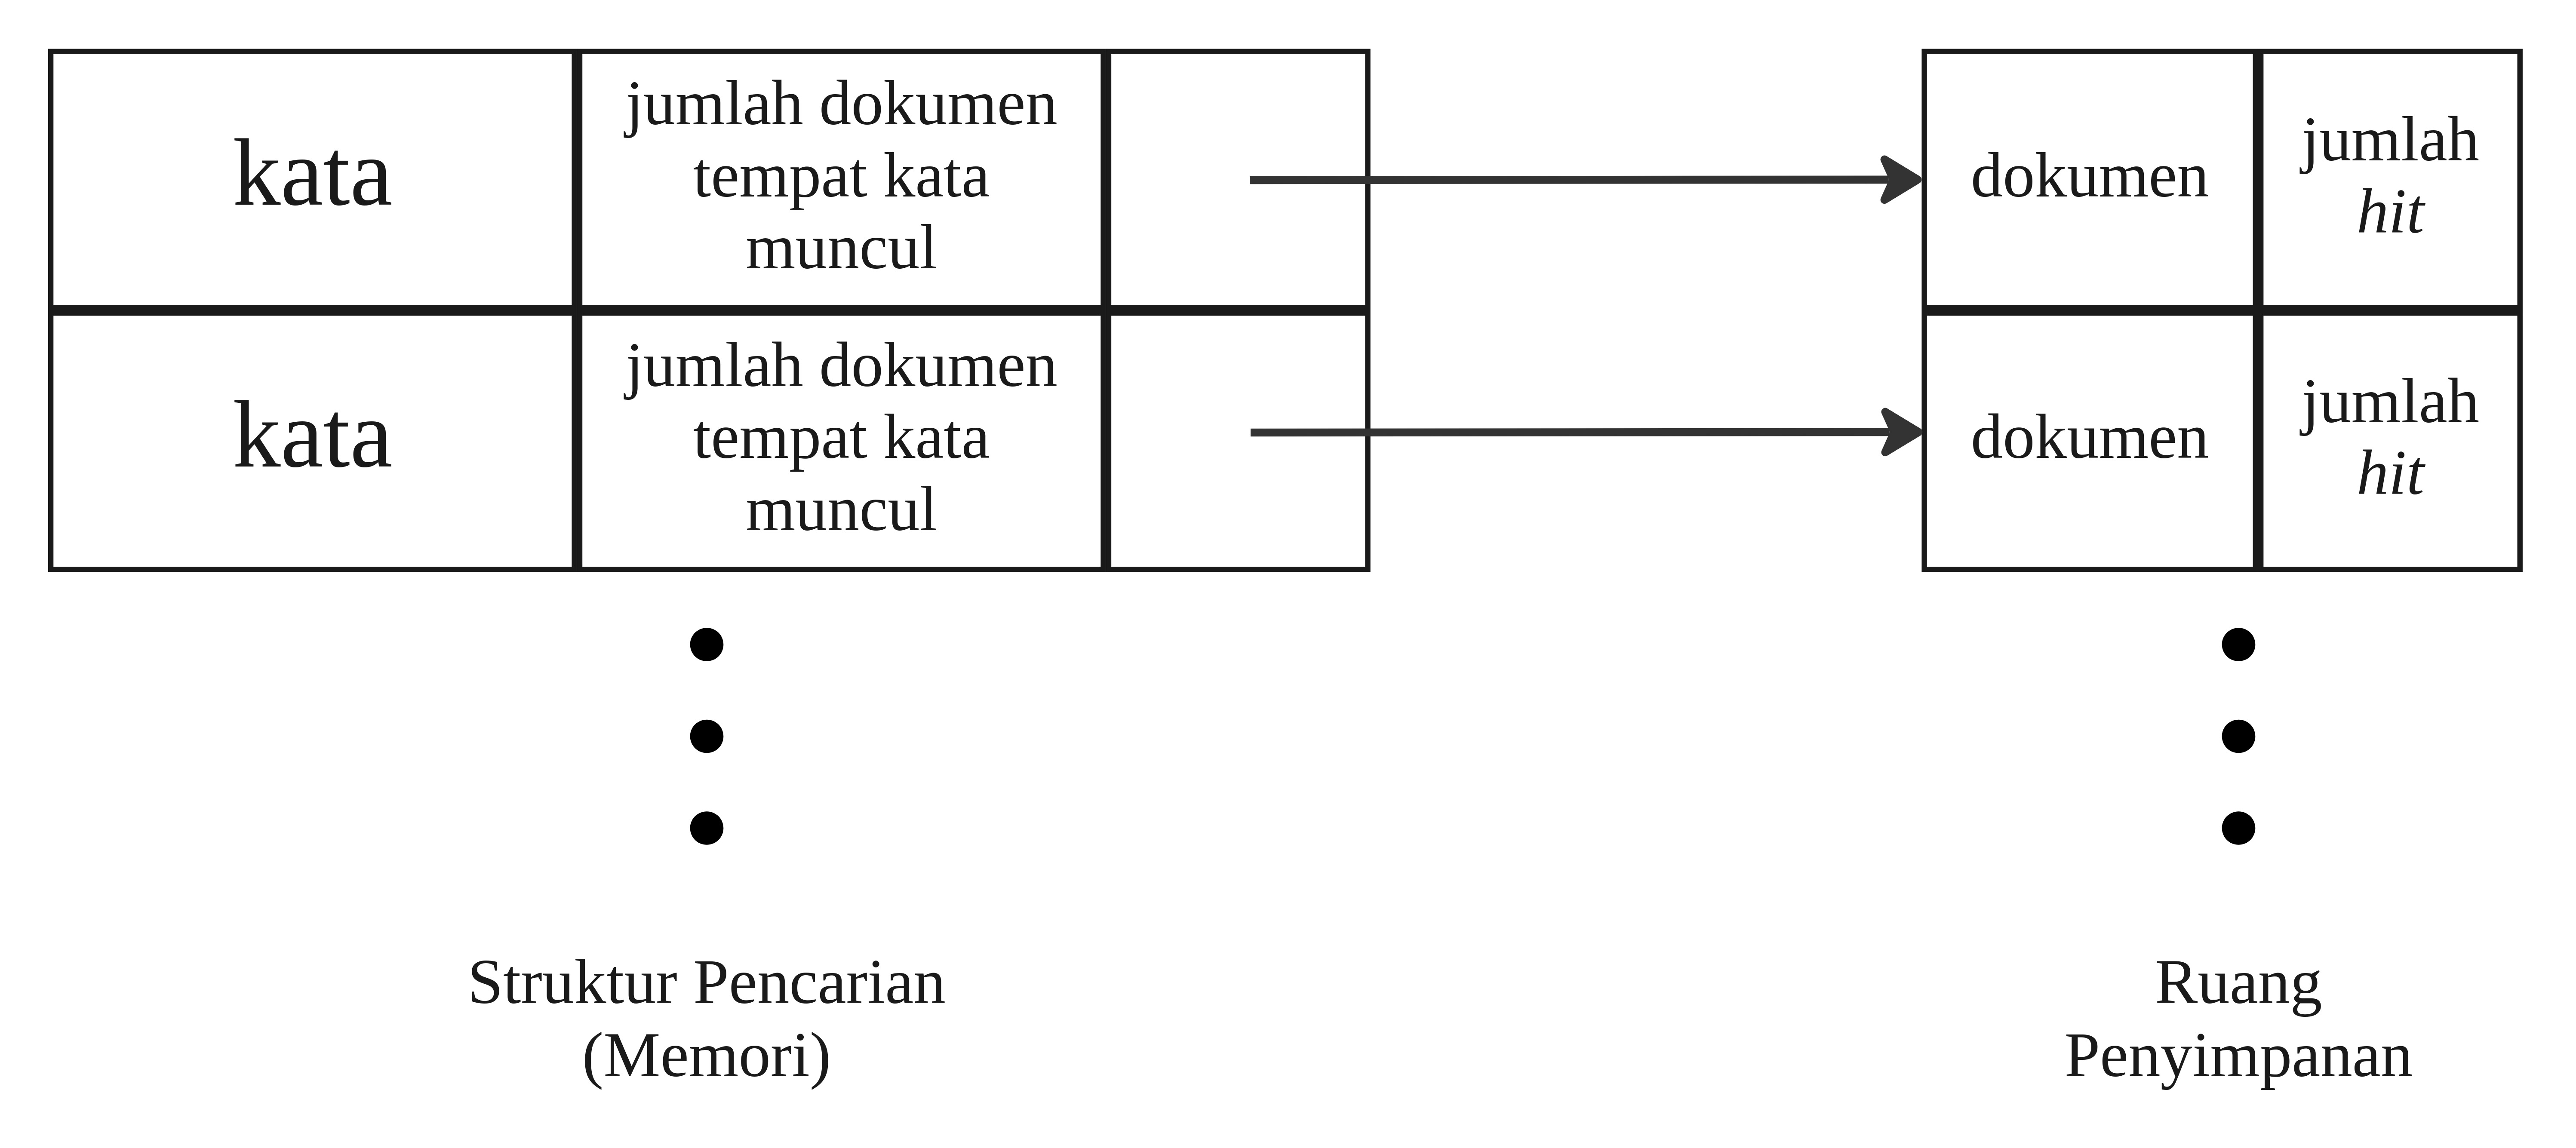
\includegraphics[width=0.85\textwidth]{gambar/hubunganStrukturPencarian}
  \caption{Penempatan jumlah \emph{hit} dalam struktur index}
\end{figure}

\subsection{Skema Penyimpanan Index}

Proses indexing akan menghasilkan \emph{forward index}, yaitu index yang telah
terurut berdasarkan \textit{id} dari dokumen. Untuk membuat \textit{inverted
index}, data pada \textit{forward index} akan diurutkan berdasarkan \textit{id}
dari kosakata.

Kemudian, dibuat dua salinan dari daftar index. Salinan pertama berisi daftar
\emph{hit} yang termasuk dalam kategori \emph{fancy hit} atau \emph{anchor hit}.
Salinan kedua adalah daftar \emph{hit} sisanya. Hal ini bertujuan untuk
mengurangi kemungkinan akses dari index, karena pada sebagian besar kasus query
dapat dipenuhi dengan hanya mengakses data pada \emph{fancy hit} dan
\emph{anchor hit}.

Pada contoh kasus mesin pencari, jumlah data di seluruh internet yang terus
bertambah membuat potensi penggunaan media penyimpanan menjadi hampir tidak
terbatas. Hal tersebut dapat menyebabkan tidak cukupnya kapasitas memori untuk
menampung seluruh index. Untuk mengatasinya, skema penyimpanan index perlu di
partisi menjadi beberapa bagian.

Selain itu, pada tiap salinan index, index juga akan di sortir berdasarkan
\emph{id} dari dokumen. Tujuannya adalah untuk memudahkan proses \emph{merging}
ketika dihadapkan pada situasi dimana query memiliki banyak kata.

% \subsection{Pemeringkatan Query}
%
% Untuk memenuhi kebutuhan tambahan seperti pemeringkatan query, struktur
% pencarian perlu menampung data tambahan seperti frekuensi kemunculan kata dan
% parameter kompresi. Apabila data tersebut tidak dapat dimuat seluruhnya pada
% memori, maka struktur pencarian dapat dipecah dan disimpan sebagian pada ruang
% penyimpanan. Sebagai contoh, kata yang bersifat umum dapat disimpan pada memori
% untuk mengurangi kemungkinan akses ke ruang penyimpanan.

\section{Proses Pembuatan Index}

Sebagai contoh, pada tabel \ref{tab:lirik} digunakan sampel teks berupa lirik
lagu anak-anak. Pada kasus ini, diasumsikan bahwa setiap baris merupakan isi
dari dokumen terpisah.

\begin{center}
  \begin{longtable}{ P{0.15\textwidth{}} P{0.75\textwidth{}}}
    \caption{Contoh teks dari lirik lagu anak-anak}
    \endlastfoot{}
    \label{tab:lirik} \\
    \textbf{Dokumen} & \textbf{Teks} \\
    \hline{}
    1 & Pease porridge hot, pease porridge cold, \\
    2 & Pease porridge in the pot, \\
    3 & Nine days old. \\
    4 & Some like it hot, some like it cold, \\
    5 & Some like it in the pot, \\
    6 & Nine days old. \\
  \end{longtable}
\end{center}

Seluruh kata dalam seluruh koleksi dokumen kemudian akan diambil jumlah
kemunculannya beserta nomor dokumen tempat kata tersebut ditemukan, dan
dikumpulkan berdasarkan keunikan kata-nya.

\begin{center}
  \begin{longtable}{ P{0.1\textwidth{}} P{0.1\textwidth{}} P{0.25\textwidth{}}}
    \caption{\textit{Inverted file index} dari lirik lagu pada tabel
    \ref{tab:lirik}}
    \endlastfoot{}
    \label{tab:file_index} \\
    \textbf{Nomor} & \textbf{Kata} & \textbf{Index} \\
    \hline{}
    1 & cold & $\langle{}2; 1, 4 \rangle{}$ \\
    2 & days & $\langle{}2; 3, 6 \rangle{}$ \\
    3 & hot & $\langle{}2; 1, 4 \rangle{}$ \\
    4 & in & $\langle{}2; 2, 5 \rangle{}$ \\
    5 & it & $\langle{}2; 4, 5 \rangle{}$ \\
    6 & like & $\langle{}2; 4, 5 \rangle{}$ \\
    7 & nine & $\langle{}2; 3, 6 \rangle{}$ \\
    8 & old & $\langle{}2; 3, 6 \rangle{}$ \\
    9 & pease & $\langle{}2; 1, 2 \rangle{}$ \\
    10 & porridge & $\langle{}2; 1, 2 \rangle{}$ \\
    11 & pot & $\langle{}2; 2, 5 \rangle{}$ \\
    12 & some & $\langle{}2; 4, 5 \rangle{}$ \\
    13 & the & $\langle{}2; 2, 5 \rangle{}$ \\
  \end{longtable}
\end{center}

Hasil index pada tabel \ref{tab:file_index} merupakan bentuk
\textit{inverted file index}, yang memetakan kata ke dokumen tempat kemunculan
kata tersebut. Untuk membuat implementasi ulang modul index milik Google, maka
diperlukan index dengan granularitas yang lebih halus. Modul index milik Google
menggunakan \textit{word-level index}, dimana index juga menyimpan posisi kata
dalam dokumen. \textit{Word-level index} dapat mengatasi situasi dimana jumlah
kemunculan suatu kata dalam dokumen lebih dari satu kali.

Dengan mengabaikan detail selain posisi kata dalam dokumen, index pada tabel
\ref{tab:file_index} dapat dikembangkan menjadi seperti berikut

\begin{center}
  \begin{longtable}{ P{0.1\textwidth{}} P{0.1\textwidth{}} P{0.2\textwidth{}}}
    \caption{\textit{Word-level index} dari lirik lagu pada tabel
    \ref{tab:lirik}}
    \endlastfoot{}
    \label{tab:word_index} \\
    \textbf{Nomor} & \textbf{Kata} & \textbf{Index} \\
    \hline{}
    1 & cold & $\langle{}2; (1;6), (4;8) \rangle{}$ \\
    2 & days & $\langle{}2; (3;2), (6;2) \rangle{}$ \\
    3 & hot & $\langle{}2; (1;3), (4;4) \rangle{}$ \\
    4 & in & $\langle{}2; (2;3), (5;4) \rangle{}$ \\
    5 & it & $\langle{}2; (4;3,7), (5;3) \rangle{}$ \\
    6 & like & $\langle{}2; (4;2,6), (5;2) \rangle{}$ \\
    7 & nine & $\langle{}2; (3;1), (6;1) \rangle{}$ \\
    8 & old & $\langle{}2; (3;3), (6;3) \rangle{}$ \\
    9 & pease & $\langle{}2; (1;1,4), (2;1) \rangle{}$ \\
    10 & porridge & $\langle{}2; (1;2,5), (2;2) \rangle{}$ \\
    11 & pot & $\langle{}2; (2;5), (5;6) \rangle{}$ \\
    12 & some & $\langle{}2; (4;1,5), (5;1) \rangle{}$ \\
    13 & the & $\langle{}2; (2;4), (5;5) \rangle{}$ \\
  \end{longtable}
\end{center}

\subsection{Pengolahan Query}

Untuk query yang hanya mengandung satu kata, hasil bisa langsung didapatkan
dengan melakukan pencarian kosakata yang memenuhi query pada daftar kosakata.
Setelah ditemukan dokumen yang membuat kata yang memenuhi query tersebut diambil
dengan petunjuk dari data yang disematkan pada daftar kosakata.

Query yang melibatkan banyak kata akan memerlukan proses penggabungan hasil dari
kosakata yang sesuai. Sebagai contoh mudahnya, query yang melibatkan banyak kata
dapat digabungkan dengan menggunakan operator logika. Operator \textit{OR} akan
memberikan gabungan dari hasil. Sementara operator \textit{AND} akan memberikan
irisan dari hasil. Jika diberikan query sebagai berikut

\[
  Q_1 \;\textit{AND} \;Q_2 \;\textit{AND} \;\cdots{} \;\textit{AND} \;Q_N
\]

maka dilakukan pencarian untuk setiap dokumen yang mengandung kata yang memenuhi
seluruh rangkaian $Q_1$ hingga $Q_n$. Dari seluruh dokumen yang sesuai, maka
dicari irisan dari hasil tersebut (dokumen yang memiliki kedua query tersebut).

Sebagai contoh, dari index pada tabel \ref{tab:file_index}, apabila diberikan
query

\[
  hot\; \textit{AND} \;like
\]

maka akan didapatkan lokasi dari index dengan kosakata \textit{hot} dan
\textit{like}, yaitu $\langle{}1, 4 \rangle{}$ dan $\langle{}4, 5 \rangle{}$.
Dari data lokasi tersebut, mereka kemudian digabungkan (diambil irisannya),
sehingga didapatkan dokumen 4 yang memenuhi kedua query tersebut.

Untuk query yang mengandung banyak kata yang tidak digabungkan dengan operator
boolean, penggunaan \textit{inverted file} seperti contoh diatas akan
menimbulkan banyaknya \textit{false match} yang mengurangi kualitas hasil dari
query. \textit{False match} sendiri dapat diatas dengan melakukan pemindaian
untuk memastikan hasil dari query. Tetapi pemindaian akan mengurangi performa
keseluruhan dari proses pengambilan data.

Penggunaan \textit{word-level index} dapat menangani hal tersebut dengan
menggunakan informasi yang lebih lengkap yang tersemat pada tiap \textit{hit}.
Karena terdapat informasi terkait posisi kata dalam dokumen, jarak antara kata
dapat dibandingkan sesuai dengan query.

% \subsection{Query Multi Kata}
%
% Apabila query memiliki lebih dari satu kata, untuk memperoleh hasil yang lebih
% akurat, struktur pencarian membutuhkan data tambahan. Data tersebut adalah
% posisi kata dalam suatu dokumen. Dengan menyimpan posisi kata, dapat dilakukan
% perbandingan posisi antar kata yang terdapat pada query.

\section{Perbandingan Metode \emph{Indexing}}

\subsection{\emph{Signature File Index}}

\emph{Signature file} adalah suatu metode probabilistik yang digunakan sebagai
alternatif untuk mengindeks teks. Pada implementasi \emph{signature file},
setiap dokumen memiliki suatu \emph{descriptor}, yaitu rangkaian \emph{bit} yang
merepresentasikan konten dari dokumen. \emph{Descriptor} dibuat dengan cara
menggunakan beberapa \emph{hash function} untuk mendapatkan suatu rangkaian bit
unik yang merepresentasikan suatu kata dalam dokumen. 

Karena sifatnya yang probabilistik, \emph{descriptor} tidak dapat bersifat unik
sepenuhnya. Terdapat kemungkinan konflik antara \emph{descriptor} dari tiap
kata. Oleh karena itu, setiap hasil \emph{hashing} dari suatu kata yang sesuai
dengan \emph{descriptor} tertentu perlu diartikan sebagai suatu kemungkinan,
bukan suatu kepastian.

Untuk memastikannya, perlu dilakukan \emph{scanning} pada dokumen yang diduga
mengandung kata tersebut. Kemungkinan terjadinya konflik dapat dikurangi dengan
menggunakan lebih banyak bit, tetapi proses \emph{scanning} tetap perlu
dilakukan untuk memastikan ada atau tidaknya suatu kata.

% Signature vs Inverted
Dibandingkan dengan inverted file, signature file memiliki dua kekurangan yang
memiliki dampak langsung untuk kebutuhan mesin pencari. Yang pertama adalah
performa yang lebih lambat dalam hal pengambilan data dari database. Hal ini
dikarenakan perlunya melakukan \emph{scanning} untuk memastikan suatu kata ada
di dalam suatu dokumen. Yang kedua adalah perlunya proses yang rumit untuk
mengolah query yang mengandung disjungsi atau negasi.

Signature file memiliki satu keunggulan dibandingkan inverted file, yaitu tidak
membutuhkan penyimpanan daftar kosakata pada memori. Oleh karena itu, di masa
lalu signature file lebih umum digunakan karena alasa keterbatasan ruang
penyimpanan. Tetapi seiring berjalannya waktu, inverted file mengadopsi teknik
kompresi yang membuat keunggulan signature file ini menjadi tidak berlaku lagi.

\subsection{\emph{Bitmap Index}}

\emph{Bitmap} adalah. Bitmap menggunakan \emph{bitvector} sebagai representasi
index. Setiap kata memiliki \emph{bitvector} yang menunjukkan keberadaan kata
tersebut dalam berbagai dokumen. Panjang dari \emph{bitvector} tergantung dari
jumlah dokumen secara kesuluruhan. Konsep bitmap sangat mudah dan cepat untuk
digunakan. Tetapi, bentuk struktur \emph{bitvector} membuat kebutuhan ruang
penyimpanan menjadi sangat besar.

Karena kekurangannya dalam hal ukuran struktur data, bitmap tidak dapat
digunakan pada berbagai kebutuhan dunia nyata, terutama mesin pencari.

\subsection{\emph{WordNet}}

\emph{WordNet} adalah suatu \emph{synonym ring} yang mampu mengelompokkan kata
berdasarkan makna yang ekuivalen secara semantik. \emph{WordNet} dapat digunakan
pada proses indexing dengan harapan hasil dari pengelompokan kata yang ditemukan
dalam dokumen dapat menjadi lebih baik. Hal ini dapat memberikan peningkatan
performa dalam proses pengambilan data.

Implementasi index menggunakan \emph{WordNet} dapat digunakan sebagai pembanding
untuk metode \emph{inverted file} yang telah dijelaskan sebelumnya.

%!TEX root = ./template-skripsi.tex
%-------------------------------------------------------------------------------
%                     BAB III
%               			PEMBAHASAN
%-------------------------------------------------------------------------------

\chapter{METODOLOGI PENELITIAN}

% Disini jelasin alur gimana dapetin index
\section{Tahapan Penelitian}

Gambar \textit{flowchart} berikut mengilustrasikan proses pembuatan \textit{
inverted index} dari dataset yang ada pada database hingga ke proses pencarian
oleh pengguna.

\begin{figure}[H]
  \centering{}
	\includegraphics[width=0.6\textwidth]{gambar/metode\-penelitian}
  \caption{Flowchart tahapan penelitian modul \textit{indexing}}
\end{figure}

\textit{Modifikasi kode \textit{Telusuri}}

Data utama yang diperlukan oleh modul \textit{indexing} dari database adalah
teks yang berisi bagian informasi inti dari halaman tersebut. Umumnya, sebuah
halaman web memiliki banyak teks diluar informasi inti yang tidak diperlukan.
Oleh karena itu, ditetapkan bahwa modul \textit{indexing} hanya akan mengambil
bagian paragraf dari halaman web. Untuk mengidentifikasi sebuah paragraf, cukup
dengan mencari \textit{tag} HTML yang sesuai (\textit{<p>}).

Walaupun sudah menspesifikasikan \textit{tag} tertentu yang akan digunakan, pada
praktiknya sering ditemukan penggunaan \textit{tag} paragraf diluar informasi
inti halaman web. Selain itu, seringkali ditemukan paragraf yang memiliki
beberapa simbol yang tidak diperlukan seperti karakter \textit{newline}. Untuk
memastikan bahwa modul \textit{indexing} hanya akan membaca paragraf inti saja,
diperlukan \textit{filter} khusus untuk menghindari masuknya informasi yang
tidak diperlukan. Parameter dari penentuan informasi ini cukup beragam, dan akan
diatur sedemikian rupa pada masa pengujian.

Pada kode program mesin pencari yang telah ada saat ini, paragraf yang disimpan
masih memiliki banyak informasi yang tidak diperlukan. Untuk memudahkan
implementasi modul \textit{indexing}, maka proses \textit{filtering} akan
dilakukan pada kode mesin pencari di bagian ekstraksi informasi dari halaman
web. Akan dibuat sebuah table baru yang berisi paragraf inti saja.

\section{Konstruksi Index}

Sebelum proses \textit{indexing} dilakukan, diperlukan sebuah
\textit{hash table} pada memori. \textit{Hash table} digunakan dengan tujuan
untuk menyimpan kata secara unik dalam dokumen. Jika nantinya ditemukan lebih
dari satu kali kemunculan kata dalam dokumen yang sama, \textit{hash table}
dapat melakukan penambahan kepada \textit{value} dari kata tersebut, dan
membentuk suatu rangkaian seperti \textit{linked list}.

% baca webpage dan ekstrak metadata
Proses \textit{indexing} dimulai dengan mengambil seluruh daftar paragraf yang
tersimpan pada database yang diurutkan berdasarkan \textit{docID}. Kemudian,
setiap paragraf akan dipecah berdasarkan karakter spasi menjadi sebuah array
berisi kata. Setiap kata lalu disimpan dalam sebuah hit bersama dengan informasi
tambahan yang ada pada paragraf.

\begin{algorithm}[H]
  \caption{Operasi \textit{sorting} pada \textit{hitlist}}\label{alg:insert}
  \begin{algorithmic}
    \Function{SortHitlist}{$H$}
      \State $sorted \gets false$
      \State $i \gets 0$

      \item[] % line skip

        \Do
          \If{$i = \Call{Len}{H} - 1$}
            \If{$sorted = true$}
              \State $break$
            \Else
              \State $i \gets 0$
            \EndIf
          \EndIf

          \item[] % line skip

          \State $tempHit \gets H[i]$

          \item[] % line skip

          \If{$H[i].text > H[i+1].text$ OR
          \newline \hspace*{3.8em}$H[i].docID > H[i+1].docID$ OR
          \newline \hspace*{3.8em}$H[i].oset > H[i+1].oset$}
            \State $H[i] \gets H[i+1]$
            \State $H[i+1] \gets tempHit$
          \EndIf

          \item[] % line skip

          \State $i \gets i+1$
        \doWhile{$sorted = false$}

        \item[] % line skip

      \State \Return
    \EndFunction
  \end{algorithmic}
\end{algorithm}

\begin{algorithm}[H]
  \caption{Algoritma pembuatan index}\label{alg:index}
  \begin{algorithmic}
    \State $hitData \gets \Call{HitData}{false}$ \Comment{Inisiasi \textit{hash table}
    untuk \textit{plain} dan \textit{fancy hit}}
    \State $hitDataAnc \gets \Call{HitData}{true}$

    \item[] % line skip

    \State $docIDList \gets [..]$
    \State $pageLinking \gets [..]$
    \State $words \gets [..]$

    \item[] % line skip

    \State $docs[..] \gets \Call{GetParagraphs}{$$}$ \Comment{Paragraf dari
    \textit{database}}
    \For{$doc \in \mathcal{} docs[..]$}
      \State $docID \gets \Call{Hash}{$$doc.url, doc.crawledAt$$}$
      \State $docList \gets \Call{Append}{$$docList$$, $$docID$$}$
      \State $words[..] \gets \Call{GetWords}{$$doc$$}$ \Comment{Kata beserta
        informasinya}

      \item[] % line skip

      \For{$word \in \mathcal{} words[..]$}
        \If{$word.url \not = nil$}
          \State $pageLinking \gets \Call{Append}{\{$$doc.url$$, $$word.url$$, $$word$$\}}$
          \State $\Call{StoreHit}{$$hitDataAnc$$, $$word$$}$
        \Else
          \State $\Call{StoreHit}{$$hitData, word$$}$
        \EndIf
      \EndFor
    \EndFor

    \item[] % line skip

    \State $(W, H) \gets \Call{Split}{$$hitData$$}$
    \State $(W_{anchor}, H_{anchor}) \gets \Call{Split}{$$hitDataAnc$$}$
    \State $lexicon \gets \Call{Append}{$$lexicon$$, $$W$$}$
    \State $lexicon \gets \Call{Append}{$$lexicon$$, $$W_{anchor}$$}$
    \State $links \gets \Call{Convert}{$$anchors$$}$ \Comment{Konversi
    \textit{anchors} menjadi pasangan \textit{docID}}
  \end{algorithmic}
\end{algorithm}

Dari proses ekstraksi kosakata beserta data tambahannya, akan didapatkan
\textit{forward index} berupa daftar \textit{hit} dari dokumen.  Daftar
\textit{hit} kemudian didistribusikan ke tempat penyimpanan berdasarkan
jenisnya. Untuk \textit{fancy hit} akan ditempatkan secara khusus pada tempat
penyimpanan yang nantinya akan menjadi sumber pencarian utama. Untuk
\textit{hit} lainnya akan ditempatkan ke tempat penyimpanan umum.

% sorting forward index jadi inverted
Untuk melakukan konversi \textit{forward index} menjadi \textit{inverted index},
dilakukan proses \textit{sorting} pada \textit{forward index}. \textit{Sorting}
dilakukan berdasarkan \textit{id} dari kosakata, kemudian dilanjutkan dengan
\textit{id} dari dokumen, dan diakhiri dengan posisi kata pada dokumen. Hasil
dari proses \textit{sorting} disimpan kembali ke tempat penyimpanan dengan
kondisi sudah menjadi \textit{inverted index}.

\section{Daftar kata umum}

Untuk meningkatkan kualitas hasil pencarian, maka skema pencarian perlu
mengabaikan kata-kata yang bersifat umum. Dari hal tersebut, perlu di dapatkan
daftar kata umum dari daftar kosakata yang telah dibuat oleh modul
\textit{indexing}. Metode yang penulis gunakan untuk mendapatkan kata umum
adalah dengan melakukan \textit{sorting} terhadap seluruh daftar kosakata
berdasarkan tingkat kemunculannya secara global. Kemudian, dengan menggunakan
batasan tertentu, akan diambil sebagian persen dari kata terbanyak yang ada.

Sebagai langkah awal, penulis berencana untuk mengambil sebanyak 1\% kata
teratas sebagai kata umum. Nilai tersebut kemudian akan diatur ulang berdasarkan
hasil \textit{user testing}.

\section{Skema Pencarian}

% NOTE Bikin flowchart proses pencarian

% Parsing query
Berdasarkan input query yang diberikan oleh pengguna, query dipecah menjadi
potongan kata yang digabungkan dengan menggunakan operator \textit{boolean}.
Kemudian, untuk setiap kosakata pada query, dilakukan \textit{scanning} terhadap
daftar kosakata. Pencarian pertama kali dilakukan pada \textit{inverted index}
yang berisi \textit{fancy hit}. Jika tidak ditemukan hasil, maka pencarian akan
dilanjutkan pada daftar \textit{plain hit}.

Untuk setiap kosakata pada daftar kosakata yang sesuai dengan kosakata pada
query, akan di dapatkan rangkaian data berupa \textit{id} dari dokumen tempat
kosakata tersebut, total jumlah \textit{hit} pada dokumen serta seluruh daftar
\textit{hit} yang berhubungan dengan kosakata pada dokumen.

% \lstinputlisting[language=Python, caption=Implementasi struktur data dengan \textit{Python}]{../koding_skripsi/main.py}

Untuk setiap daftar \textit{hit} yang didapatkan, dilakukan \textit{merging}
sehingga tersisa dokumen yang memenuhi query.

\begin{algorithm}[H]
  \caption{Proses pengolahan dan pencarian \textit{query}}
  \begin{algorithmic}
    \Function{MergeHitlist}{$p1$, $p2$}
    \State $M \gets [..]$
    \While{$p1 \not = nil$ AND $p2 \not = nil$}
      % TODO Handle multiline
      \If{$p1.docID = p2.docID$} \Comment{Cek kesamaan \textit{docID}}
        \If{$-(p1.oset - p2.oset)$ = 1} \Comment{Cek selisih offset}
          \State \Call{Append}{$M$, $p1$}
        \EndIf
      \EndIf
      \State $p1 \gets \Call{next}{$p1$}$
      \State $p2 \gets \Call{next}{$p2$}$
    \EndWhile{}
    \State \Return $M$
    \EndFunction

    \item[] % line skip

    \State $H \gets [..]$
    \State $W \gets \Call{ParseQuery}{query}$ \Comment{Pecah query menjadi
    daftar kata}
    \For{$w \in \mathcal{} W$}
      \State $h \gets \Call{GetHitlist}{w}$ \Comment{Cari nilai $w$ pada daftar
      kosakata secara sekuensial}
      \If{$h = nil$}
        \State continue
      \EndIf
      \State \Call{Append}{H, h}
    \EndFor

    \item[] % line skip

    \State $i \gets 0$
    \While{$i \not = \Call{Len}{H}$}
      \State $H[0] = \Call{MergeHitlist}{$H[0]$, $H[i]$}$
      \State $i \gets i + 1$
    \EndWhile

    \item[] % line skip

    \State $result \gets \Call{GetResult}{H[0]}$
  \end{algorithmic}
\end{algorithm}

\section{Metode Pemeringkatan}

Dari hasil rangkaian \textit{hit} yang didapatkan, perlu dilakukan beberapa
operasi untuk mendapatkan urutan hasil dokumen yang paling sesuai. Hasil
peringkat yang didapatkan dilakukan berdasarkan dua faktor berikut

\begin{itemize}
  \item{\textit{Word similarity ($\beta$)}, yaitu kemunculan hasil yang memenuhi beberapa
    bagian dari query}
  \item{\textit{Word distance ($\gamma$)}, yaitu jarak kata yang memenuhi query}
\end{itemize}

\subsection{\textit{Word similarity ($\beta$)}}

\textit{Word similarity} menilai suatu kata berdasarkan kemiripannya dari kata
pada query. Untuk membandingkan apakah suatu kata memiliki makna atau maksud
yang sama dengan kata lainnya, akan digunakan \textit{Jaccard distance}.
Perbandingan akan dilakukan berdasarkan hasil kombinasi pada seluruh karakter
yang ada pada kosakata untuk membuat pasangan dua huruf.

Karena \textit{Jaccard distance} mengukur nilai ketidakmiripan dari dua model,
maka tinggi nilai $\beta$ maka nilai dokumen akan semakin rendah.

% TODO Contoh perbandingan dengan Jaccard

\subsection{\textit{Word distance ($\gamma$)}}

Perhitungan \textit{word distance} digunakan untuk melakukan validasi terhadap
urutan kata yang muncul pada dokumen. Urutan dari kata berpengaruh terhadap
maksud dari query. Selain itu, jarak yang terlalu jauh antara kata yang
ditemukan dapat mengurangi relevansi informasi.

Untuk membandingkan jarak kata, seluruh kata pada query perlu diberikan urutan
yang sesuai dengan menggunakan angka terlebih dahulu. Setelah \textit{hitlist}
didapatkan, posisi dari kata yang ditemukan akan dikurangi dengan posisi asli
pada query. Nilai dari dokumen bisa didapatkan dengan rumus

\begin{equation}
  D = (|(L_1 - \acute{L_1})| + |(L_2 - \acute{L_2})| + ... + |(L_n - \acute{L_n})|) - ((L_1 - \acute{L_1}) \times N)
\end{equation}

dimana

\begin{conditions}
  N & Jumlah kata pada query \\
  L_n & Posisi awal kata ke-$n$ pada query \\
  \acute{L_n} & Posisi kata ke-$n$ pada query di dokumen
\end{conditions}

\subsection{Rumus akhir}

Dari seluruh faktor prioritas diatas, maka nilai dari suatu dokumen bisa
didapatkan dengan rumus

\begin{equation}
  \text{TODO Rumus akhir} \\
  D = \lambda_1 S + \lambda_2 S + ... + \lambda_n S
\end{equation}

dimana

\begin{conditions}
  D & Skor dokumen \\
  N & Jumlah kata pada query \\
  Q_n & Query ke-$n$ \\
\end{conditions}

\section{Alat dan Bahan Penelitian}

Pada penelitian ini, terdapat beberapa alat yang digunakan sebagai penunjang
dalam pembuatan modul \textit{indexing} dengan rincian sebagai berikut:

\begin{itemize}
  \item{Laptop HP Elitebook 840 G5 (Intel Core i5-8250U, 16GB RAM)}
  \item{Sistem operasi \textit{Linux}}
  \item{\textit{Neovim} sebagai \textit{code editor}}
  \item{\textit{Podman} untuk menjalankan database \textit{MySQL}}
  \item{Python 3.10}
\end{itemize}

\section{Tahapan Pengembangan}

\subsection{Meningkatkan kemampuan modul \textit{indexing} saat ini}

Pencarian akan dilakukan secara sekuensial terhadap daftar index yang telah
dihasilkan oleh modul \textit{indexing}. Sebagai pembanding, hasil dari
penelitian ini akan digabungkan dengan hasil penelitian Zaidan berjudul \textit{
PERANCANGAN MODUL PENGINDEKS PADA SEARCH ENGINE BERUPA GENERALIZED SUFFIX TREE
UNTUK KEPERLUAN PEMERINGKATAN DOKUMEN}.

Hasil penelitian tersebut menghasilkan modul \textit{indexing} dengan bentuk
\textit{Generalized Suffix Tree (GST)}. Penggunaan modul \textit{GST} dapat
langsung memberikan hasil berupa dokumen tempat kata tersebut berada. Dengan
demikian, modul index pada penelitian ini hanya perlu menunjukkan lokasi kata
pada dokumen melalui informasi yang ada pada \textit{hit}.

Tetapi karena hasil penelitian Zaidan masih memiliki kendala ketika dilakukan
ujicoba secara independen oleh penulis, maka akan dilakukan implementasi ulang
dengan menggunakan modul \textit{GST} yang tersedia di internet.

% TODO Flowchart kalo misalnya jadi pake GST

\subsection{Integrasi pada arsitektur \textit{Telusuri}}

Modul \textit{indexing} akan diintegrasikan dengan mesin pencari
\textit{Telusuri} dalam bentuk API. Hal ini dikarenakan modul ini akan terlibat
dalam proses pemeringkatan hasil pencarian.

% TODO Buat menjelaskan tentang skema pengujian apa yang akan digunakan
% biar ketauan kalo penelitiannya berguna
% \section{Pengujian}

%!TEX root = ./template-skripsi.tex
%-------------------------------------------------------------------------------
%                            	BAB IV
%               		KESIMPULAN DAN SARAN
%-------------------------------------------------------------------------------

\chapter{UJI COBA DAN HASIL UJI COBA}

\section{Uji Coba}
Uji coba sistem dilakukan terhadap 30 responden anggota KOPMA UNJ dengan rincian, \textit{admin} yang terdiri dari 2 responden, pengawas yang terdiri dari 3 responden, dan anggota yang terdiri dari 25 responden. Setiap responden akan melakukan uji coba terhadap sistem yang dibuat berdasarkan peran masing-masing responden. Uji coba yang dilakukan menggunakan data dari hasil sebaran kuesioner \textit{User Acceptance Test}. \textit{User Acceptance Test} bertujuan untuk mengetahui perihal sistem yang dikembangkan apakah sudah sesuai dengan kebutuhan \textit{user} atau belum. Skala yang digunakan dalam penelitian ini adalah skala \textit{likert}.

Langkah-langkah pengujian sistem informasi Koperasi Mahasiswa Universitas Negeri Jakarta yang akan dilakukan adalah sebagai berikut:
\begin{enumerate}
	\item \textit{User} melakukan pendaftaran anggota.
	\item \textit{Admin} melakukan verifikasi penerimaan anggota.
	\item \textit Seluruh \textit{user} dapat mengelola biodata pribadi.
	\item \textit{Admin} mengelola status keanggotaan setiap \textit{user} (\textit{admin}, pengawas, atau anggota biasa).
	\item Anggota dan pengawas yang sudah memiliki akun dapat mengakses ke dalam sistem sesuai berandanya masing-masing.
	\item \textit{Admin} menambahkan data barang, stok, simpanan, transaksi anggota, dan keuangan.
	\item Data yang \textit{admin} tambahkan akan muncul dan dapat dilihat di beranda semua \textit{user}.
	\item \textit{Admin} mengelola (sunting dan hapus) data barang, stok, simpanan, transaksi anggota, dan keuangan.
	\item Data yang \textit{admin} kelola akan berubah dan dapat dilihat di beranda semua \textit{user}.	
	\item Pengawas menambahkan data penilaian untuk KOPMA UNJ.
	\item Data yang pengawas tambahkan akan muncul dan dapat dilihat di beranda  semua \textit{user}.
	\item Pengawas mengelola (sunting dan hapus) data penilaian untuk KOPMA UNJ.
	\item Data yang pengawas kelola akan berubah dan dapat dilihat di beranda semua \textit{user}.	
\end{enumerate}

Fitur milik setiap \textit{user} yang akan diuji pada sistem informasi Koperasi Mahasiswa Universitas Negeri Jakarta adalah sebagai berikut:

\begin{itemize}
	\item \textit{Admin}
	\begin{enumerate}
		\item Masuk ke dalam sistem
		\item Penyuntingan data pribadi
		\item Pengelolaan anggota (tambah, kesesuaian \textit{id}, detail, pemutihan, sunting, \textit{reset password}, tambah periode, pengelompokan, pemulihan, keuangan anggota, dan cetak)
		\item Pengelolaan barang (tambah, sunting, hapus, cetak, dan pengelompokan)
		\item Pengelolaan stok (tambah, hapus, dan cetak)
		\item Pengelolaan simpanan (tambah, hapus, cetak, dan pengelompokan)
		\item Pengelolaan transaksi (tambah, hapus, dan cetak)
		\item Transparansi penilaian
		\item Pengelolaan dan kesesuaian arus keuangan (tambah dana tambahan dan beban lain)
		\item Pengelolaan \textit{admin} (tambah dan hapus \textit{admin})
		\item Pengelolaan pengawas (tambah dan hapus pengawas)
		\item Pengelolaan penerimaan anggota (terima dan tolak anggota)
		\item Keluar dari sistem
	\end{enumerate}

	\item Anggota
	\begin{enumerate}
		\item Melakukan pendaftaran
		\item Masuk ke dalam sistem
		\item Penyuntingan data pribadi
		\item Transparansi data (barang, stok, transaksi, penilaian, dan arus keuangan)
		\item Keluar dari sistem
	\end{enumerate}
	
	\item Pengawas
	\begin{enumerate}
		\item Masuk ke dalam sistem
		\item Penyuntingan data pribadi
		\item Transparansi data (barang, stok, transaksi, dan arus keuangan)
		\item Pengelolaan penilaian (tambah, sunting, hapus, dan cetak)
		\item Keluar dari sistem
		\end{enumerate}
	\end{itemize}

Semua fitur yang diuji memiliki penilaian yang dirincikan menjadi beberapa kategori. Data kuantitatif akan dianalisis dengan menggunakan skala \textit{ likert}. Berikut kategori dan skor penilaian dalam tahap pengujian\textit{ User Acceptance Test} pada sistem informasi Koperasi Mahasiswa Universitas Negeri Jakarta dengan menggunakan skala \textit{likert}:\\

\begin{tabular}{lll}
SS& = Sangat Setuju& diberikan nilai 5\\
S& = Setuju& diberikan nilai 4\\
C& = Cukup& diberikan nilai 3\\
TS& = Tidak Setuju& diberikan nilai 2\\
STS& = Sangat Tidak Setuju& diberikan nilai 1\\
\\
\end{tabular}

Kemudian hasil pendataan yang telah didapatkan dengan teknik penyebaran angket dikalkulasikan dengan menggunakan sistem penilaian sebagai berikut:

\begin{itemize}
	\item Nilai total
	
	Nilai total merupakan nilai dari hasil perhitungan antara responden kuesioner angket dengan nilai di setiap poin pertanyaan. Berikut merupakan rumus nilai total:
	
	\textit{Nilai total = jumlah nilai setiap soal}
	
	\item Nilai rata-rata
	
	Nilai rata-rata merupakan nilai dari hasil perhitungan antara nilai total dengan jumlah responden yang mengisi kuesioner angket. Berikut merupakan rumus dari nilai rata-rata:

	\textit{Nilai rata-rata = nilai total / jumlah responden}
	
\end{itemize}

Untuk mengetahui kualitas produk yang dikembangkan layak atau tidak, maka perlu ditentukan dengan menghitung seluruh nilai rata-rata dari setiap pertanyaan. Nilai tersebut kemudian akan dibandingkan dengan interpretasi skor pada skala \textit{likert}. Analisis data yang disajikan ke distribusi skor dan persentase terhadap kategori menggunakan interpretasi skor untuk skala \textit{likert}. Berikut rentang interpretasi skor untuk skala \textit{likert}:\\

\begin{tabular}{lll}
	Nilai& = 0\% - 20\%& Sangat Kurang Sesuai \\
	Nilai& = 21\% - 40\%& Kurang Sesuai\\
	Nilai& = 41\% - 60\%& Cukup Sesuai\\
	Nilai& = 61\% - 80\%& Sesuai\\
	Nilai& = 81\% - 100\%& Sangat Sesuai\\
\end{tabular}

\section{Hasil Uji Coba}
Berdasarkan hasil uji coba \textit{User Acceptance Test} yang dilakukan terhadap 30 anggota KOPMA UNJ, yakni \textit{admin} yang terdiri dari 2 responden, pengawas terdiri dari 3 responden, dan anggota terdiri dari 25 responden, diperoleh hasil uji coba sebagai berikut:

\subsection{\textit{Admin}}
Berikut merupakan daftar pertanyaan \textit{User Acceptance Test} pada \textit{Admin}:

\begin{table}[H]
	\centering
	\caption{Daftar Pertanyaan \textit{User Acceptance Test} pada \textit{Admin}}
	\includegraphics[width=1.0\textwidth]{gambar/Tabel_Admin1}
\end{table}

\begin{table}[H]
	\centering
	\caption{Daftar Pertanyaan \textit{User Acceptance Test} pada \textit{Admin}}
	\includegraphics[width=1.0\textwidth]{gambar/Tabel_Admin2}
\end{table}

Setelah kuisioner \textit{admin} diberikan kepada responden, kemudian data kuesioner diolah untuk mendapatkan hasil penilaian \textit{user acceptance test}. Adapun hasil penilaian \textit{user acceptance test} tersebut yaitu:

\begin{table}[H]
	\centering
	\caption{Data Hasil Penyebaran Kuesioner \textit{User Acceptance Test} pada \textit{Admin}}
	\includegraphics[width=1\textwidth]{gambar/Hasil_Admin}
\end{table}

Dari hasil penilaian pengujian \textit{user acceptance test} dapat diambil kesimpulan yaitu:

\begin{enumerate}
	\item Pengguna sistem yang telah memilih Sangat Tidak Setuju (STS) memiliki persentase 0\%
	\item Pengguna sistem yang telah memilih Tidak Setuju (TS) memiliki persentase 0\%
	\item Pengguna sistem yang telah memilih Cukup (C) memiliki persentase 8\%.
	\item Pengguna sistem yang telah memilih Setuju (S) memiliki persentase 57\%.
	\item Pengguna sistem yang telah memilih Sangat Setuju (SS) memiliki persentase 35\%.
	\item Rata-rata penerimaan \textit{user} adalah 4,27 dari 5 atau sekitar 85\%.
\end{enumerate}

\begin{figure}[H]
	\centering
	\includegraphics[width=1\textwidth]{gambar/Grafik_Admin}
	\caption{Grafik Hasil Penyebaran Kuesioner \textit{User Acceptance Test} pada \textit{Admin}}
\end{figure}

Berdasarkan hasil pengujian \textit{user acceptance test} yang diujikan kepada 2 responden \textit{admin}, dapat dilihat bahwa secara keseluruhan 35\% menjawab sangat setuju, 57\% menjawab setuju, 8\% menjawab cukup, serta rata-rata penerimaan \textit{user} terhadap kesesuaian sistem dengan kebutuhan adalah 4,27 dari 5 atau sekitar 85\%, oleh karena itu dapat diambil kesimpulan bahwa fitur yang \textit{admin} butuhkan dalam sistem informasi yang dirancang sudah sangat sesuai dengan kebutuhan dan berjalan dengan baik.  

\subsection{\textit{Anggota}}
Berikut merupakan daftar pertanyaan \textit{User Acceptance Test} pada Anggota

\begin{table}[H]
	\centering
	\caption{Daftar Pertanyaan \textit{User Acceptance Test} pada Anggota}
	\includegraphics[width=1\textwidth]{gambar/Tabel_Anggota}
\end{table}

Setelah kuisioner anggota diberikan kepada responden, kemudian data kuesioner diolah untuk mendapatkan hasil penilaian \textit{user acceptance test}. Adapun hasil penilaian \textit{user acceptance test} tersebut yaitu:

\begin{table}[H]
	\centering
	\caption{Data Hasil Penyebaran Kuesioner \textit{User Acceptance Test} pada Anggota}
	\includegraphics[width=1\textwidth]{gambar/Hasil_Anggota}
\end{table}

Dari hasil pengujian \textit{user acceptance test} dapat diambil kesimpulan yaitu:

\begin{enumerate}
	\item Pengguna sistem yang telah memilih Sangat Tidak Setuju (STS) memiliki persentase 0\%
	\item Pengguna sistem yang telah memilih Tidak Setuju (TS) memiliki persentase 0\%
	\item Pengguna sistem yang telah memilih Cukup (C) memiliki persentase 23\%.
	\item Pengguna sistem yang telah memilih Setuju (S) memiliki persentase 58\%.
	\item Pengguna sistem yang telah memilih Sangat Setuju (SS) memiliki persentase 19\%.
	\item Rata-rata penerimaan \textit{user} adalah 3,96 dari 5 atau sekitar 79\%.
\end{enumerate}

\begin{figure}[H]
	\centering
	\includegraphics[width=1\textwidth]{gambar/Grafik_Anggota}
	\caption{Grafik Hasil Penyebaran Kuesioner \textit{User Acceptance Test} pada Anggota}
\end{figure}

Berdasarkan hasil pengujian \textit{user acceptance test} yang diujikan kepada 25 responden anggota, dapat dilihat bahwa secara keseluruhan 19\% menjawab sangat setuju, 58\% menjawab setuju, 23\% menjawab cukup, serta rata-rata penerimaan \textit{user} terhadap kesesuaian sistem dengan kebutuhan adalah 3,96 dari 5 atau sekitar 79\%, oleh karena itu dapat diambil kesimpulan bahwa fitur yang anggota butuhkan dalam sistem informasi yang dirancang sudah sesuai dengan kebutuhan dan berjalan dengan baik. 
\\
\\
\\
\\
\\

\subsection{\textit{Pengawas}}
Berikut merupakan daftar pertanyaan \textit{User Acceptance Test} pada Pengawas

\begin{table}[H]
	\centering
	\caption{Daftar Pertanyaan \textit{User Acceptance Test} pada Pengawas}
	\includegraphics[width=1\textwidth]{gambar/Tabel_Pengawas}
\end{table}

Setelah kuisioner pengawas diberikan kepada responden, kemudian data kuesioner diolah untuk mendapatkan hasil penilaian \textit{user acceptance test}. Adapun hasil penilaian \textit{user acceptance test tersebut} tersebut yaitu:

\begin{table}[H]
	\centering
	\caption{Data Hasil Penyebaran Kuesioner \textit{User Acceptance Test} pada Pengawas}
	\includegraphics[width=1\textwidth]{gambar/Hasil_Pengawas}
\end{table}

Dari hasil penilaian pengujian \textit{user acceptance test} dapat diambil kesimpulan yaitu:

\begin{enumerate}
	\item Pengguna sistem yang telah memilih Sangat Tidak Setuju (STS) memiliki persentase 0\%
	\item Pengguna sistem yang telah memilih Tidak Setuju (TS) memiliki persentase 0\%
	\item Pengguna sistem yang telah memilih Cukup (C) memiliki persentase 2\%.
	\item Pengguna sistem yang telah memilih Setuju (S) memiliki persentase 42\%.
	\item Pengguna sistem yang telah memilih Sangat Setuju (SS) memiliki persentase 56\%.
	\item Rata-rata penerimaan \textit{user} adalah 4,53 dari 5 atau sekitar 91\%.
\end{enumerate}

\begin{figure}[H]
	\centering
	\includegraphics[width=1\textwidth]{gambar/Grafik_Pengawas}
	\caption{Grafik Hasil Penyebaran Kuesioner \textit{User Acceptance Test} pada Pengawas}
\end{figure}

Berdasarkan hasil pengujian \textit{user acceptance test} yang diujikan kepada 3 responden pengawas, dapat dilihat bahwa secara keseluruhan 56\% menjawab sangat setuju, 42\% menjawab setuju, 2\% menjawab cukup, serta rata-rata penerimaan \textit{user} terhadap kesesuaian sistem dengan kebutuhan adalah 4,53 dari 5 atau sekitar 91\%, oleh karena itu dapat diambil kesimpulan bahwa fitur yang pengawas butuhkan dalam sistem informasi yang dirancang sudah sangat sesuai dengan kebutuhan dan berjalan dengan baik. 

% Baris ini digunakan untuk membantu dalam melakukan sitasi
% Karena diapit dengan comment, maka baris ini akan diabaikan
% oleh compiler LaTeX.
\begin{comment}
\bibliography{daftar-pustaka}
\end{comment}
%!TEX root = ./template-skripsi.tex
%-------------------------------------------------------------------------------
%                          BAB V
%               		KESIMPULAN DAN SARAN
%-------------------------------------------------------------------------------

\chapter{KESIMPULAN DAN SARAN}

\section{Kesimpulan}

Berdasarkan hasil dari implementasi dan pengujian terhadap arsitektur
\textit{inverted index}, maka diperoleh kesimpulan sebagai berikut:

\begin{enumerate}
	\item{Data pada kolom \textit{paragraph} dengan jumlah 1.010.083 baris dari
		tabel \textit{page\_paragraph} berhasil digunakan untuk membuat struktur
		\textit{inverted index}.}
	\item{Modul \textit{indexer} berbasis \textit{inverted index} yang digunakan
		untuk melakukan pemeringkatan pada \textit{query} yang diberikan oleh 
		pengguna telah selesai dibuat.}
	\item{Penyimpanan persisten untuk struktur \textit{inverted index} 
		diimplementasikan sebagai penyimpanan sederhana dalam satu proses yang sama 
		dengan modul \textit{indexer}.}
	\item{Integrasi dengan struktur \textit{GST} yang telah dibuat pada penelitian 
		sebelumnya berhasil diintegrasikan dengan struktur \textit{inverted index}.}
	\item{Integrasi dengan struktur \textit{GST} dapat memberikan reduksi waktu 
		pencarian yang signifikan jika dibandingkan hanya dengan penggunaan
		\textit{inverted index} saja, dengan rasio perbedaan berkisar antara 85 
		- 98\%.}
	\item{Relevansi pencarian tidak terlalu baik jika hanya menggunakan
		\textit{inverted index}. Hasil menjadi lebih relevan ketika menggunakan 
		integrasi \textit{GST}.}
	\item{Informasi yang ada pada \textit{tag} paragraf (\textit{<p>}) tidak cukup 
		untuk menjadi dasar dalam pemeringkatan hasil pencarian.}
\end{enumerate}

\section{Saran}

Adapun saran untuk penelitian selanjutnya adalah:
\begin{enumerate} 
	\item{Melanjutkan penelitian tentang informasi lain yang dapat di ekstrak dari 
		suatu halaman web untuk meningkatkan hasil pencarian.}
	\item{Melakukan perombakan terhadap struktur \textit{hitlists} agar bisa 
		direferensikan melalui alamat memori untuk menghilangkan redundansi pada 
		struktur dengan integrasi \textit{GST}.}
	\item{Melanjutkan penelitian tentang penggunaan kompresi pada struktur
		\textit{hit} untuk mereduksi penggunaan memori.}
	\item{Menuliskan implementasi \textit{indexer} dengan menggunakan bahasa lain 
		yang lebih cepat dan mampu mengeksploitasi sistem \textit{multi-thread} 
		dengan lebih baik seperti \textit{Rust} atau \textit{C++}.}
	\item{Melanjutkan penelitian tentang distribusi penyimpanan dan penggunaan 
		\textit{hitlists} pada memori.}
\end{enumerate}


% Baris ini digunakan untuk membantu dalam melakukan sitasi
% Karena diapit dengan comment, maka baris ini akan diabaikan
% oleh compiler LaTeX.
\begin{comment}
\bibliography{daftar-pustaka}
\end{comment}


%-----------------------------------------------------------------
%Disini akhir masukan Bab
%-----------------------------------------------------------------


%-----------------------------------------------------------------
% Disini awal masukan untuk Daftar Pustaka
% - Daftar pustaka diambil dari file .bib yang ada pada folder ini
%   juga.
% - Untuk memudahkan dalam memanajemen dan menggenerate file .bib
%   gunakan reference manager seperti Mendeley, Zotero, EndNote,
%   dll.
%-----------------------------------------------------------------
% \bibliography{daftar-pustaka}
% \bibliographystyle{apalike}
\addcontentsline{toc}{chapter}{DAFTAR PUSTAKA}
\singlespacing{}
\printbibliography{}
%-----------------------------------------------------------------
%Disini akhir masukan Daftar Pustaka
%-----------------------------------------------------------------

\addcontentsline{toc}{chapter}{LAMPIRAN}
\appendix 
\chapter{Dokumentasi Pengujian Metode \textit{Inverted Index}}
\begin{figure}[H]
	\centering
	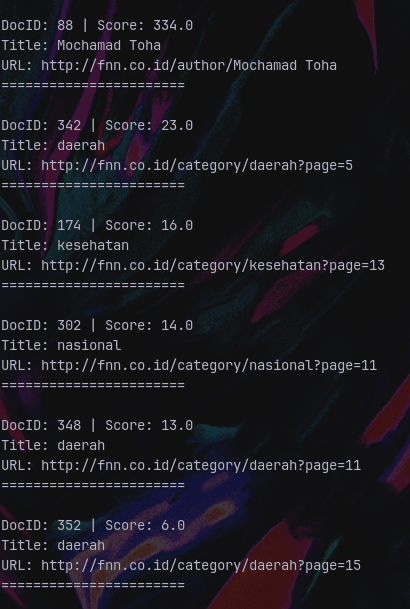
\includegraphics[width=0.95\textwidth]{gambar/hasil_inv_bupati}	
\end{figure}

\chapter{Dokumentasi Pengujian Metode \textit{Inverted Index} dan Integrasi \textit{GST}}
\begin{figure}[H]
	\centering
	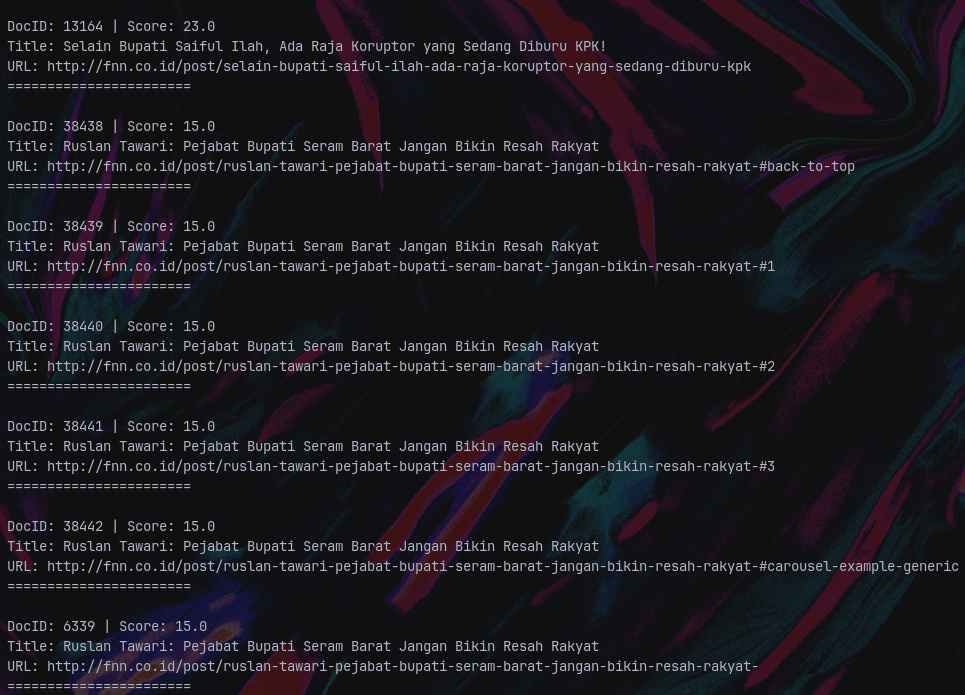
\includegraphics[width=0.95\textwidth]{gambar/hasil_gst_bupati}	
\end{figure}

\pagestyle{empty}
\chapter*{\centering \large DAFTAR RIWAYAT HIDUP}
\thispagestyle{empty}

\begin{wrapfigure}{l}{4cm}
	\vspace{-25pt}
	\begin{center}
		\includegraphics[width=0.27\textwidth]{gambar/pas-foto}
	\end{center}
	\vspace{-80pt}
\end{wrapfigure}

\noindent \textbf{MUHAMMAD YAN HANDOKO.}  Lahir di Semarang, 18 Juni 1997.  Anak pertama dari pasangan Bapak Muhammad dan Ibu Siti Wafirotun. Saat ini beralamatkan di Jl. Pengadegan Barat V RT.011 RW.007 No.18, Pancoran Jakarta Selatan.

\vspace{0.5cm}
\noindent
\begin{center}
	\begin{flushright}
		\begin{tabular}{lcl}
			No. Ponsel	& :&  082124022340 \\
			Email	& :&  myanhandkoko17@gmail.com
		\end{tabular}
	\end{flushright}
\end{center}
\vspace{0.5cm}

\noindent \textbf{Riwayat Pendidikan} : Penulis mengawali pendidikan di SDN Pengadegan 08 Pengadegan Pagi pada tahun 2002 - 2008. Setelah itu, penulis melanjutkan studi ke SMPN 154 Jakarta hingga tahun 2011. Kemudian melanjutkan ke SMAN 43 Jakarta pada tahun 2011-2014. Di Tahun 2014 penulis melanjutkan ke Universitas Negeri Jakarta (UNJ), Program Studi Ilmu Komputer, melalui jalur PENMABA. Di awal tahun 2019 (Senin, 18 Februari 2019) penulis telah memperoleh gelar Sarjana Komputer (S.Kom), Program Studi Ilmu Komputer, Fakultas Matematika dan Ilmu Pengetahuan Alam, Universitas Negeri Jakarta.

\noindent \textbf{Riwayat Organisasi} : Selama di bangku perkuliahan, penulis aktif di Badan Eksekutif Mahasiswa Jurusan Matematika sebagai staff Departemen Kaderisasi periode 2015-2016, Badan Eksekutif Mahasiswa Rumpun Matematika sebagai Ketua periode 2016-2017, Badan Eksekutif Mahasiswa Fakultas Matematika dan Ilmu Pengetahuan Alam sebagai Ketua periode 2017-2018, dan Badan Eksekutif Mahasiswa Universitas Negeri Jakarta sebagai Kepala Departemen Kaderisasi periode 2018. Penulis juga berpartisipasi dalam organisasi keilmiahan di Program Studi Ilmu Komputer yaitu DEFAULT, dimana penulis tergabung sebagai anggota divisi \textit{web}. Penulis juga tergabung dengan organisasi kemahasiswaan lain seperti, Masjid Ulul Albaab sebagai staff MUA \textit{Media Center} periode 2015, Desa Binaan FMIPA UNJ sebagai pengajar periode 2015-2016 dan kepala divisi informasi dan komunikasi periode 2015-2016, Tim Aksinya Kampus MIPA sebagai staff pusat pergerakan periode 2016-2017. Penulis juga kerap mengikuti kepanitiaan kegiatan yang diadakan oleh lembaga eksekutif (BEM), lembaga legislatif (LLM), dan lembaga dakwah fakultas (MUA), dan komunitas/\textit{underbow} lembaga (Default, Desa Binaan, TAnK MIPA). 


\end{document}
